% MICRO 2026 Survey Paper - ML Performance Models
% Using MICRO 59 ACM sigconf template
% Last compiled: 2026-02-07 (rebuild triggered)

%%
%% For submission and review of your manuscript please change the
%% command to \documentclass[manuscript, screen, review]{acmart}.
%%
\documentclass[sigconf, screen, review]{acmart}

%%
%% \BibTeX command to typeset BibTeX logo in the docs
\AtBeginDocument{%
  \providecommand\BibTeX{{%
    Bib\TeX}}}

%% Rights management information - for submission
\setcopyright{none}
\copyrightyear{2026}
\acmYear{2026}
\acmDOI{}

%% Conference information
\acmConference[MICRO 2026]{The 59th IEEE/ACM International Symposium on Microarchitecture}{November 2026}{Austin, TX, USA}
\acmISBN{}

%% Disable ACM reference format printing for submission
\settopmatter{printfolios=true}
\settopmatter{printacmref=false}

%% Anonymous submission
\author{Anonymous Author(s)}
\affiliation{%
  \institution{Under Review}
  \country{Anonymous}
}

%% Additional packages (acmart already loads amsmath, amsfonts, amssymb, booktabs)
\usepackage{multirow}
\usepackage{tikz}
\usetikzlibrary{shapes.geometric,arrows.meta,positioning,fit,backgrounds,patterns}
\usepackage{pgfplots}
\pgfplotsset{compat=1.18}
\usepgfplotslibrary{groupplots}
\usetikzlibrary{plotmarks}

% Custom commands
\newcommand{\todo}[1]{\textcolor{red}{[TODO: #1]}}

\begin{document}

\title{A Survey of High-Level Modeling and Simulation Methods for Modern Machine Learning Workloads}
\subtitle{\normalsize{MICRO 2026 Submission -- Confidential Draft -- Do NOT Distribute!!}}

%%
%% The abstract is a short summary of the work to be presented in the
%% article.

%%%%%% -- PAPER CONTENT STARTS-- %%%%%%%%

\begin{abstract}
As machine learning workloads grow in scale and complexity---spanning training and inference for CNNs, transformers, mixture-of-experts models, and LLMs---architects and system designers need fast, accurate methods to predict their performance across diverse hardware platforms.
This survey provides a comprehensive analysis of the tools and methods available for modeling and simulating the performance of ML workloads, covering analytical models, cycle-accurate simulators, trace-driven approaches, and ML-augmented hybrid techniques.
We survey over 30 tools drawn from 53 papers across architecture venues (MICRO, ISCA, HPCA, ASPLOS) and systems venues (MLSys, OSDI, NSDI) published between 2016--2026, spanning DNN accelerator modeling (Timeloop, MAESTRO, Sparseloop), GPU simulation (GPGPU-Sim, Accel-Sim, NeuSight), distributed training simulation (ASTRA-sim, Lumos, SimAI), and LLM inference serving (VIDUR, Frontier, AMALI).
We organize the literature along three dimensions---methodology type (analytical, simulation, ML-augmented, hybrid), target platform (accelerators, GPUs, distributed systems, edge devices), and abstraction level (kernel, model, system)---while additionally characterizing tools by workload coverage, revealing a pervasive CNN-validation bias.
Our analysis reveals that hybrid approaches combining analytical structure with learned components achieve the best accuracy-speed trade-offs, while pure analytical models offer superior interpretability for design space exploration.
We conduct hands-on reproducibility evaluations of five representative tools, finding that reproducibility varies dramatically: Docker-first tools score 8.5+/10 on our rubric while tools relying on serialized ML models risk becoming unusable.
We identify key open challenges including cross-workload generalization beyond CNNs, composition of kernel-level predictions to end-to-end accuracy, and support for emerging architectures.
This survey provides practitioners guidance for selecting appropriate modeling tools and researchers a roadmap for advancing the field of ML workload performance prediction.
\end{abstract}

%%
%% Keywords
\keywords{ML workload performance prediction, DNN accelerator modeling, GPU simulation, distributed training simulation, LLM inference serving, design space exploration, survey}

\maketitle

% ==============================================================================
% INTRODUCTION
% ==============================================================================
\section{Introduction}
\label{sec:introduction}

Machine learning workloads---spanning training and inference for CNNs, transformers, mixture-of-experts models, and graph neural networks---have become the dominant consumers of compute across datacenters and edge devices.
The shift toward domain-specific architectures~\cite{hennessy2019golden}, from Google's TPU~\cite{tpuv1_2017,tpuv4_2023} to custom training accelerators, has created a heterogeneous hardware landscape where architects and system designers need fast, accurate performance predictions to navigate vast design spaces, select parallelization strategies, provision serving infrastructure, and optimize hardware-software co-design.
Yet ML workloads pose unique modeling challenges: they exhibit diverse computational patterns (dense matrix operations in attention layers, sparse accesses in GNNs, communication-bound collective operations in distributed training) across this increasingly heterogeneous landscape of GPUs, TPUs, custom accelerators, and multi-device clusters.

A rich ecosystem of modeling and simulation tools has emerged to address these challenges, spanning a methodological spectrum from analytical models to cycle-accurate simulators to ML-augmented hybrid approaches.
Analytical frameworks like Timeloop~\cite{timeloop2019} and MAESTRO~\cite{maestro2019} model DNN accelerator performance through closed-form data movement analysis, achieving 5--10\% error versus RTL at microsecond evaluation speed.
Cycle-accurate simulators like GPGPU-Sim~\cite{gpgpusim2009} and Accel-Sim~\cite{accelsim2020} provide detailed GPU modeling but require hours per workload.
Trace-driven simulators like ASTRA-sim~\cite{astrasim2023} and VIDUR~\cite{vidur2024} target distributed training and LLM serving at system scale.
ML-augmented approaches like NeuSight~\cite{neusight2025} learn performance functions from profiling data, achieving 2.3\% error on GPU kernel prediction.
Each methodology occupies a distinct point in the accuracy-speed-generality trade-off space.

Despite this rich tool landscape, no comprehensive survey organizes these methods from the perspective of the ML workload practitioner---the architect or engineer who needs to select a modeling tool for a specific design or deployment task.
Existing surveys focus on ML \emph{techniques} for performance modeling~\cite{granite2022} or on specific hardware targets~\cite{timeloop2019}, leaving practitioners without guidance on which tools suit their needs across the full modeling spectrum.
This survey fills that gap by providing a methodology-centric view of the tools and methods available for predicting ML workload performance.

We make the following contributions:
\begin{itemize}
    \item A \textbf{methodology-centric taxonomy} organizing tools along three dimensions: methodology type (analytical, simulation, ML-augmented, hybrid), target platform (DNN accelerators, GPUs, distributed systems, edge devices), and abstraction level (kernel, model, system), with a quantitative coverage matrix identifying research gaps and a workload coverage analysis exposing the CNN-validation bias in the literature.
    \item A \textbf{systematic survey} of over 30 modeling tools drawn from 53 papers across architecture venues (MICRO, ISCA, HPCA, ASPLOS) and systems venues (MLSys, OSDI, NSDI) published between 2016--2026, using documented selection criteria.
    \item A \textbf{comparative analysis} examining trade-offs between accuracy, speed, generalization, and interpretability, with careful qualification of paper-reported accuracy claims and identification of cases where reported numbers are unverifiable.
    \item \textbf{Hands-on reproducibility evaluations} of representative tools with a 10-point rubric, and identification of \textbf{open challenges} including the CNN-to-transformer generalization gap, kernel-to-end-to-end error composition, and emerging accelerator support.
\end{itemize}

The remainder of this paper is organized as follows.
Section~\ref{sec:methodology} describes our survey methodology and positions this work relative to existing surveys.
Section~\ref{sec:background} provides background on ML workload characteristics and modeling fundamentals.
Section~\ref{sec:taxonomy} presents our classification taxonomy.
Section~\ref{sec:survey} surveys approaches organized by target platform.
Section~\ref{sec:comparison} offers comparative analysis across key dimensions and a practitioner tool selection guide.
Section~\ref{sec:evaluation} presents hands-on reproducibility evaluations.
Section~\ref{sec:challenges} discusses open challenges and future directions.
Section~\ref{sec:conclusion} concludes.

Figure~\ref{fig:timeline} illustrates the evolution of performance modeling tools for ML workloads, from early analytical frameworks through simulators to modern hybrid approaches.

\begin{figure}[t]
\centering
\resizebox{\columnwidth}{!}{%
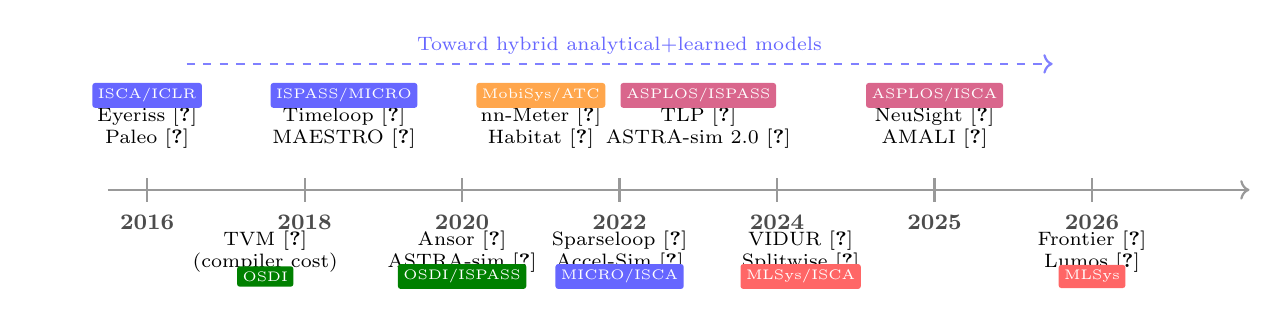
\begin{tikzpicture}[
    node distance=0.3cm,
    yearnode/.style={font=\footnotesize\bfseries, text=black!70},
    eventnode/.style={font=\scriptsize, text width=2.8cm, align=center},
    catnode/.style={font=\tiny, text=white, rounded corners=1pt, inner sep=2pt}
]
% Timeline base
\draw[thick, ->, black!40] (0,0) -- (14.5,0);

% Year markers
\foreach \x/\year in {0.5/2016, 2.5/2018, 4.5/2020, 6.5/2022, 8.5/2024, 10.5/2025, 12.5/2026} {
    \draw[thick, black!40] (\x,-0.15) -- (\x,0.15);
    \node[yearnode, below] at (\x,-0.2) {\year};
}

% Events - staggered heights to avoid overlap
% 2016: Eyeriss, Paleo
\node[eventnode, above] at (0.5,0.4) {Eyeriss~\cite{eyeriss2016}\\Paleo~\cite{paleo2017}};
\node[catnode, fill=blue!60] at (0.5,1.2) {ISCA/ICLR};

% 2018: TVM
\node[eventnode, below] at (2.0,-0.4) {TVM~\cite{tvm2018}\\(compiler cost)};
\node[catnode, fill=green!50!black] at (2.0,-1.1) {OSDI};

% 2019: Timeloop, MAESTRO
\node[eventnode, above] at (3.0,0.4) {Timeloop~\cite{timeloop2019}\\MAESTRO~\cite{maestro2019}};
\node[catnode, fill=blue!60] at (3.0,1.2) {ISPASS/MICRO};

% 2020: Ansor, ASTRA-sim
\node[eventnode, below] at (4.5,-0.4) {Ansor~\cite{ansor2020}\\ASTRA-sim~\cite{astrasim2020}};
\node[catnode, fill=green!50!black] at (4.5,-1.1) {OSDI/ISPASS};

% 2021: nn-Meter, Habitat
\node[eventnode, above] at (5.5,0.4) {nn-Meter~\cite{nnmeter2021}\\Habitat~\cite{habitat2021}};
\node[catnode, fill=orange!70] at (5.5,1.2) {MobiSys/ATC};

% 2022: Sparseloop
\node[eventnode, below] at (6.5,-0.4) {Sparseloop~\cite{sparseloop2022}\\Accel-Sim~\cite{accelsim2020}};
\node[catnode, fill=blue!60] at (6.5,-1.1) {MICRO/ISCA};

% 2023: TLP, ASTRA-sim 2.0
\node[eventnode, above] at (7.5,0.4) {TLP~\cite{tlp2023}\\ASTRA-sim 2.0~\cite{astrasim2023}};
\node[catnode, fill=purple!60] at (7.5,1.2) {ASPLOS/ISPASS};

% 2024: VIDUR, Splitwise
\node[eventnode, below] at (8.8,-0.4) {VIDUR~\cite{vidur2024}\\Splitwise~\cite{splitwise2024}};
\node[catnode, fill=red!60] at (8.8,-1.1) {MLSys/ISCA};

% 2025: NeuSight, AMALI, SimAI
\node[eventnode, above] at (10.5,0.4) {NeuSight~\cite{neusight2025}\\AMALI~\cite{amali2025}};
\node[catnode, fill=purple!60] at (10.5,1.2) {ASPLOS/ISCA};

% 2026: Frontier, Dynamic Reasoning
\node[eventnode, below] at (12.5,-0.4) {Frontier~\cite{frontier2025}\\Lumos~\cite{lumos2025}};
\node[catnode, fill=red!60] at (12.5,-1.1) {MLSys};

% Trend arrow
\draw[thick, ->, blue!50, dashed] (1,1.6) -- (12,1.6);
\node[font=\scriptsize, text=blue!60, above] at (6.5,1.6) {Toward hybrid analytical+learned models};

\end{tikzpicture}
}
\caption{Evolution of performance modeling tools for ML workloads (2016--2026). Early analytical frameworks (Eyeriss, Paleo) gave way to systematic accelerator modeling (Timeloop, MAESTRO) and distributed training simulation (ASTRA-sim). ML-augmented approaches (TVM, Habitat, NeuSight) learn performance functions from data. Recent work targets LLM-specific modeling (VIDUR, AMALI, Frontier) and large-scale training prediction (Lumos).}
\label{fig:timeline}
\end{figure}

% ==============================================================================
% SURVEY METHODOLOGY
% ==============================================================================
\section{Survey Methodology}
\label{sec:methodology}

We follow a systematic methodology for identifying, selecting, and classifying papers in this survey.

\textbf{Search strategy.}
We searched ACM Digital Library, IEEE Xplore, Semantic Scholar, and arXiv using terms including ``performance modeling DNN,'' ``DNN accelerator simulator,'' ``LLM inference prediction,'' ``distributed training simulation,'' ``neural network latency estimation,'' and ``ML workload performance.''
We additionally performed backward/forward citation tracking from seminal works (Timeloop, ASTRA-sim, NeuSight) and monitored proceedings of target venues.

\textbf{Target venues.}
Architecture: MICRO, ISCA, HPCA, ASPLOS.
Systems: MLSys, OSDI, SOSP, NSDI.
Related: NeurIPS, ICML, MobiSys, DAC, ISPASS.

\textbf{Inclusion criteria.}
Papers must (1)~propose or evaluate a tool or method for predicting performance of ML workloads (training or inference), (2)~target at least one hardware platform (GPU, accelerator, distributed system, or edge device), and (3)~include quantitative evaluation of prediction accuracy or modeling fidelity.

\textbf{Exclusion criteria.}
We exclude (1)~papers using ML for non-performance tasks (e.g., power estimation without latency), (2)~papers modeling general-purpose (non-ML) workloads exclusively, and (3)~papers without quantitative evaluation.

\textbf{Selection process.}
Our initial search yielded 287 candidate papers.
After title/abstract screening against inclusion criteria, 118 remained.
Full-text review reduced the set to 53 papers that met all criteria.
We additionally include 12 foundational works (gem5, roofline model, DRAMSim, etc.) as context for understanding the modeling landscape.

\textbf{Time period.}
We cover papers published between 2016--2026, with foundational works from earlier years included for context.

\textbf{Classification.}
We classify each paper along three dimensions: \emph{methodology type} (analytical, cycle-accurate simulation, trace-driven simulation, ML-augmented, or hybrid), \emph{target platform} (DNN accelerator, GPU, distributed system, edge device, or CPU), and \emph{abstraction level} (kernel/operator, model/end-to-end, or system).
We additionally characterize each tool by workload coverage, prediction targets, and reported accuracy metrics.

\subsection{Related Surveys}
\label{subsec:related-surveys}

Several surveys address adjacent topics.
In the ML-for-systems space, Rakhshanfar and Zarandi~\cite{rakhshanfar2021survey} survey ML techniques for processor design space exploration, focusing on surrogate model construction rather than the tools available to ML practitioners.
Sze et al.~\cite{sze2017efficient} provide a comprehensive treatment of DNN hardware architectures and dataflow optimization, establishing the conceptual framework on which analytical tools like Timeloop and MAESTRO are built; however, their scope is DNN accelerator design rather than cross-platform performance prediction.
In GPU simulation, the gem5-gpu~\cite{binkert2011gem5} and GPGPU-Sim~\cite{gpgpusim2009} ecosystems have generated extensive evaluation literature, but no survey organizes GPU, accelerator, distributed, and edge modeling tools within a unified taxonomy.
The MLPerf benchmark suites~\cite{mlperf_training2020,mlperf_inference2020} standardize ML workload measurement across hardware but focus on \emph{measurement} rather than \emph{prediction}---they provide ground truth data that performance models should target but do not survey the modeling tools themselves.
Hennessy and Patterson~\cite{hennessy2019golden} frame the current era as a ``new golden age'' for domain-specific architectures, motivating the need for performance prediction tools that span the heterogeneous hardware landscape, but do not survey these tools.

This survey differs from prior work in three ways: (1)~it spans the full methodology spectrum from analytical to ML-augmented, rather than focusing on a single approach; (2)~it covers all major target platforms (accelerators, GPUs, distributed systems, edge devices) rather than a single hardware class; and (3)~it includes hands-on reproducibility evaluations that go beyond paper-reported accuracy claims.
The closest prior work is the latency predictor study by Dudziak et al.~\cite{latencypredictorsnas2024}, which systematically compares edge device predictors for NAS; we broaden the scope to the full platform and methodology landscape.

% ==============================================================================
% BACKGROUND
% ==============================================================================
\section{Background}
\label{sec:background}

This section provides background on the characteristics of ML workloads that make performance modeling challenging, and reviews the fundamental approaches used to model them.

\subsection{ML Workload Characteristics}
\label{subsec:workload-characteristics}

ML workloads present unique performance modeling challenges compared to general-purpose programs.
Modern ML frameworks like PyTorch~\cite{pytorch2019} and TensorFlow~\cite{tensorflow2016} define workloads as computation graphs of operators, providing a structured representation that performance models can exploit.

\textbf{Computational structure.}
ML workloads are composed of well-defined operators (convolutions, matrix multiplications, attention layers, normalization) with statically known shapes and data types.
This regularity enables analytical modeling of compute and data movement, unlike branch-heavy general-purpose code.
However, modern architectures like mixture-of-experts (MoE) and dynamic inference introduce input-dependent control flow that complicates static analysis.

\textbf{Memory hierarchy sensitivity.}
DNN accelerators employ specialized memory hierarchies with explicit data orchestration.
The mapping of tensor operations to hardware (dataflow, tiling, loop ordering) critically determines performance.
For LLM inference, KV cache management dominates memory behavior, with cache sizes scaling linearly with sequence length and batch size~\cite{vllm2023}.

\textbf{Scale and distribution.}
Large model training distributes computation across thousands of GPUs using data, tensor, pipeline, and expert parallelism~\cite{llama3scaling2025}.
Performance depends on the interplay between compute, memory bandwidth, and network communication---requiring system-level modeling beyond single-device prediction.

\textbf{Distinct inference phases.}
LLM inference exhibits qualitatively different phases: prefill (compute-bound, processing the full prompt) and decode (memory-bound, generating tokens autoregressively)~\cite{splitwise2024}.
Effective modeling must capture both phases and their interaction under batched serving~\cite{sarathi2024,orca2022}.

\subsection{Modeling Methodologies}
\label{subsec:modeling-methodologies}

We classify modeling approaches into four categories that form the primary axis of our taxonomy.

\textbf{Analytical models} express performance as closed-form functions of workload and hardware parameters.
The roofline model~\cite{williams2009roofline} bounds throughput by $P = \min(\pi, \beta \cdot I)$, where $\pi$ is peak compute, $\beta$ is memory bandwidth, and $I$ is operational intensity.
For DNN accelerators, Timeloop~\cite{timeloop2019} analytically computes data movement costs across memory hierarchies for any valid mapping.
Analytical models provide microsecond evaluation and full interpretability, but require manual derivation per architecture and struggle with dynamic microarchitectural effects.

\textbf{Cycle-accurate simulators} model hardware at the register-transfer level.
gem5~\cite{binkert2011gem5} (CPUs), GPGPU-Sim~\cite{gpgpusim2009} (GPUs), and Accel-Sim~\cite{accelsim2020} (modern GPUs) achieve detailed accuracy but suffer $1000$--$10000\times$ slowdown, making them impractical for full ML workload evaluation.
Sampling techniques (SimPoint~\cite{simpoint2002}, SMARTS~\cite{smarts2003}) reduce simulation time but were designed for general-purpose workloads and may not capture ML-specific patterns.

\textbf{Trace-driven simulation} uses execution traces as input rather than full binary execution, enabling faster evaluation.
ASTRA-sim~\cite{astrasim2023} models distributed training using Chakra execution traces~\cite{chakra2023} with pluggable compute, memory, and network backends.
VIDUR~\cite{vidur2024} provides discrete-event simulation for LLM serving using kernel-level profiles.
This approach trades some fidelity for orders-of-magnitude speedup over cycle-accurate simulation.

\textbf{ML-augmented approaches} learn performance functions from profiling data.
These range from simple models (random forests in nn-Meter~\cite{nnmeter2021}, XGBoost in TVM~\cite{tvm2018}) to deep learning (NeuSight~\cite{neusight2025}) and meta-learning (HELP~\cite{help2021}).
ML-augmented approaches can capture complex non-linear relationships that elude analytical treatment, but require training data and may not generalize beyond their training distribution.

\subsection{Problem Formulation}
\label{subsec:problem-formulation}

Performance modeling maps workload $\mathcal{W}$ and hardware $\mathcal{H}$ to a performance metric $y$: $\hat{y} = f(\mathcal{W}, \mathcal{H}; \theta)$.
Workloads are represented at operator level (layer parameters), graph level (computation graphs), IR level (compiler representations), or trace level (recorded runtime behavior).
Hardware is characterized by specifications, performance counters, or learned embeddings.

\textbf{Prediction targets} include latency (execution time), throughput (samples/second), energy (Joules per inference), and memory footprint.
Multi-objective formulations enable Pareto-optimal design selection.

\textbf{Accuracy metrics} vary across the literature: MAPE (scale-invariant relative error), RMSE (penalizes large deviations), and rank correlation (Kendall's $\tau$) for design space ordering.
Direct comparison across papers is limited by differences in benchmarks, hardware targets, and evaluation protocols---a challenge we discuss in Section~\ref{sec:comparison}.

% ==============================================================================
% TAXONOMY
% ==============================================================================
\section{Taxonomy}
\label{sec:taxonomy}

We organize the literature along three dimensions.
The \emph{primary axis} is methodology type---how a tool predicts performance---because methodology determines the fundamental trade-offs between accuracy, speed, interpretability, and data requirements.
The \emph{secondary axes} are target platform and abstraction level, which together determine the scope and applicability of each tool.
We additionally characterize tools by workload coverage, exposing a pervasive CNN-validation bias in the literature.

Figure~\ref{fig:taxonomy-overview} illustrates the primary and secondary dimensions.
Table~\ref{tab:taxonomy-matrix} provides a unified view combining the coverage matrix (number of surveyed tools per methodology--platform cell) with trade-off profiles (evaluation speed, data requirements, interpretability, and failure modes), with empty cells highlighting research gaps.

\begin{figure}[t]
\centering
\resizebox{\columnwidth}{!}{%
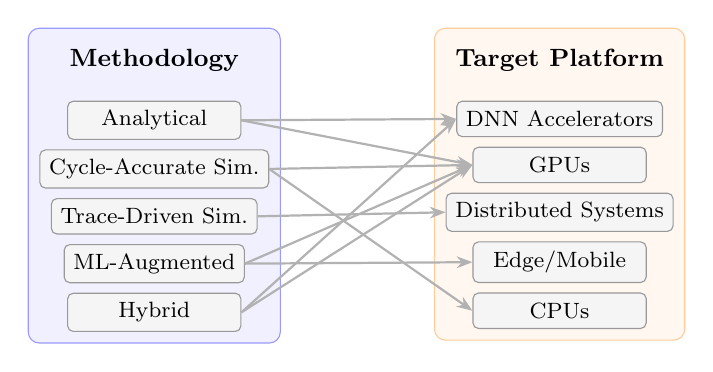
\begin{tikzpicture}[
    node distance=0.4cm and 0.6cm,
    catbox/.style={rectangle, rounded corners=2pt, draw=black!40, fill=gray!8, minimum width=2.2cm, minimum height=0.45cm, font=\footnotesize},
    dimlabel/.style={font=\small\bfseries, text=black},
    arrow/.style={-{Stealth[length=2mm]}, thick, draw=black!50}
]

% === METHODOLOGY TYPE (Left column) ===
\node[dimlabel] (meth-label) at (0, 0) {Methodology};
\node[catbox, below=0.25cm of meth-label] (analytical) {Analytical};
\node[catbox, below=0.12cm of analytical] (cycleacc) {Cycle-Accurate Sim.};
\node[catbox, below=0.12cm of cycleacc] (tracedriven) {Trace-Driven Sim.};
\node[catbox, below=0.12cm of tracedriven] (mlaugmented) {ML-Augmented};
\node[catbox, below=0.12cm of mlaugmented] (hybrid) {Hybrid};

% === TARGET PLATFORM (Right column) ===
\node[dimlabel, right=2.5cm of meth-label] (hw-label) {Target Platform};
\node[catbox, below=0.25cm of hw-label] (accel) {DNN Accelerators};
\node[catbox, below=0.12cm of accel] (gpu) {GPUs};
\node[catbox, below=0.12cm of gpu] (dist) {Distributed Systems};
\node[catbox, below=0.12cm of dist] (edge) {Edge/Mobile};
\node[catbox, below=0.12cm of edge] (cpu) {CPUs};

% === Connecting arrows showing tool-method pairings ===
% Analytical -> Accelerators (Timeloop, MAESTRO)
\draw[arrow, black!30] (analytical.east) -- (accel.west);
% Analytical -> GPU (AMALI, Roofline)
\draw[arrow, black!30] (analytical.east) -- (gpu.west);
% Cycle-accurate -> GPU (GPGPU-Sim, Accel-Sim)
\draw[arrow, black!30] (cycleacc.east) -- (gpu.west);
% Cycle-accurate -> CPU (gem5)
\draw[arrow, black!30] (cycleacc.east) -- (cpu.west);
% Trace-driven -> Distributed (ASTRA-sim, Lumos)
\draw[arrow, black!30] (tracedriven.east) -- (dist.west);
% ML-augmented -> Edge (nn-Meter, LitePred)
\draw[arrow, black!30] (mlaugmented.east) -- (edge.west);
% ML-augmented -> GPU (TVM, Ansor)
\draw[arrow, black!30] (mlaugmented.east) -- (gpu.west);
% Hybrid -> GPU (NeuSight)
\draw[arrow, black!30] (hybrid.east) -- (gpu.west);
% Hybrid -> Accelerators (ArchGym)
\draw[arrow, black!30] (hybrid.east) -- (accel.west);

% === Background boxes for each dimension ===
\begin{scope}[on background layer]
    \node[fit=(meth-label)(analytical)(cycleacc)(tracedriven)(mlaugmented)(hybrid), fill=blue!6, draw=blue!40, rounded corners=4pt, inner sep=4pt] {};
    \node[fit=(hw-label)(accel)(gpu)(dist)(edge)(cpu), fill=orange!6, draw=orange!40, rounded corners=4pt, inner sep=4pt] {};
\end{scope}

\end{tikzpicture}%
}
\caption{Taxonomy of ML workload performance modeling along two of three dimensions (methodology type and target platform; abstraction level is detailed in \S\ref{subsec:by-abstraction}). Arrows show dominant pairings: analytical models for accelerators, cycle-accurate simulation for GPUs/CPUs, trace-driven simulation for distributed systems, and ML-augmented approaches for edge devices and compiler cost models.}
\label{fig:taxonomy-overview}
\end{figure}

% --- Unified Taxonomy Table (merged from Tables 1+2, issue #192) ---
\begin{table*}[t]
\centering
\caption{Methodology taxonomy: coverage matrix and trade-off profile.
Platform columns show the number of surveyed tools per cell; \textbf{0} indicates an explicit research gap.
Speed, data requirements, and interpretability determine practical applicability; the failure mode column identifies the primary condition under which each methodology breaks down.}
\label{tab:taxonomy-matrix}
\small
\begin{tabular}{l|ccccc|cccc}
\toprule
 & \textbf{DNN} & & \textbf{Distrib.} & \textbf{Edge/} & & \textbf{Eval.} & \textbf{Data} & & \textbf{Failure} \\
\textbf{Methodology} & \textbf{Accel.} & \textbf{GPU} & \textbf{Systems} & \textbf{Mobile} & \textbf{CPU} & \textbf{Speed} & \textbf{Req.} & \textbf{Interp.} & \textbf{Mode} \\
\midrule
Analytical       & 3 & 3 & 2 & \textbf{0} & \textbf{0} & $\mu$s & None & High & Dynamic effects \\
Cycle-Accurate   & 1 & 2 & \textbf{0} & \textbf{0} & 1 & Hours & Binary & High & Scale \\
Trace-Driven     & \textbf{0} & \textbf{0} & 7 & \textbf{0} & \textbf{0} & Min. & Traces & Med. & Trace fidelity \\
ML-Augmented     & \textbf{0} & 3 & \textbf{0} & 3 & 1 & ms & Profiling & Low & Distrib.\ shift \\
Hybrid           & 1 & 3 & \textbf{0} & \textbf{0} & 1 & ms & Mixed & Med. & Training domain \\
\bottomrule
\end{tabular}
\end{table*}

Table~\ref{tab:taxonomy-matrix} reveals three structural observations.
First, trace-driven simulation is exclusively used for distributed systems---no surveyed tool applies trace-driven methods to single-device GPU or accelerator modeling, despite the potential for trace-driven approaches to avoid the slowdown of cycle-accurate simulation while retaining more fidelity than analytical models.
Second, edge/mobile devices are served exclusively by ML-augmented approaches; the absence of analytical or hybrid models for edge devices reflects the hardware diversity problem but also represents a research gap, since hybrid approaches could combine the interpretability of analytical models with the adaptability of learned components.
Third, no ML-augmented or hybrid tool specifically targets distributed system modeling---tools like VIDUR use ML internally for kernel prediction but are architecturally trace-driven simulators.
The trade-off columns further show that methodologies cluster into two speed regimes: sub-millisecond (analytical, ML-augmented, hybrid) suitable for design space exploration, and minutes-to-hours (simulation, trace-driven) suitable for detailed validation.

\subsection{Primary Axis: Methodology Type}
\label{subsec:by-methodology}

The choice of methodology determines fundamental trade-offs between accuracy, evaluation speed, data requirements, and interpretability, as summarized in the right columns of Table~\ref{tab:taxonomy-matrix}.

\subsubsection{Analytical Models}

Analytical models express performance as closed-form functions of workload and hardware parameters.
For DNN accelerators, Timeloop~\cite{timeloop2019} models data movement across memory hierarchies for any valid loop-nest mapping, achieving 5--10\% error versus RTL at 2000$\times$ speedup.
MAESTRO~\cite{maestro2019} provides data-centric dataflow analysis using intuitive directives.
Sparseloop~\cite{sparseloop2022} extends to sparse tensor operations.
Paleo~\cite{paleo2017} pioneered layer-wise analytical modeling for DNNs, decomposing networks into compute and communication components for distributed training prediction.
AMALI~\cite{amali2025} targets LLM inference on GPUs through improved memory hierarchy modeling.

Analytical models provide microsecond evaluation, full interpretability, and ``what-if'' design analysis.
Their limitation is that they require manual derivation per architecture and may miss complex dynamic effects (e.g., memory contention, scheduling variability).
AMALI's 23.6\% MAPE illustrates the accuracy ceiling of analytical approaches for complex GPU workloads---the residual error stems from dynamic microarchitectural effects that resist closed-form treatment (see \S\ref{subsec:gpu-modeling} for detailed analysis).

\subsubsection{Cycle-Accurate Simulation}

Cycle-accurate simulators model hardware at register-transfer level, providing the highest fidelity.
gem5~\cite{binkert2011gem5} (CPUs), GPGPU-Sim~\cite{gpgpusim2009} (GPUs), and Accel-Sim~\cite{accelsim2020} (modern NVIDIA GPUs, SASS-level trace-driven) achieve 0.90--0.97 IPC correlation.
PyTorchSim~\cite{pytorchsim2025} integrates PyTorch 2 with NPU simulation supporting custom RISC-V ISA and systolic arrays.

The primary limitation is speed: simulating a single ResNet-50 inference may require hours, making these tools impractical for design space exploration of ML workloads.
Simulation sampling techniques (SimPoint~\cite{simpoint2002}, SMARTS~\cite{smarts2003}, LoopPoint~\cite{looppoint2022}) accelerate general-purpose workload simulation but are not specifically validated for ML workload patterns.
Recent work on dissecting modern GPU cores~\cite{dissectinggpu2025} has improved Accel-Sim's accuracy to 13.98\% MAPE by reverse-engineering undocumented microarchitectural details.
Note that the 0.90--0.97 IPC \emph{correlation} metric can coexist with 20\%+ absolute latency error for workloads with atypical occupancy patterns---correlation captures relative ordering fidelity but not absolute prediction accuracy.

\subsubsection{Trace-Driven Simulation}

Trace-driven approaches use recorded execution traces rather than full binary execution, enabling system-level modeling at practical speeds.
ASTRA-sim~\cite{astrasim2023} models distributed training end-to-end using Chakra execution traces~\cite{chakra2023}, with pluggable compute, memory, and network backends, achieving 5--15\% error versus real clusters.
Echo~\cite{echo2024} simulates distributed training at scale using analytical compute models with network simulation.
Lumos~\cite{lumos2025} targets LLM training performance through trace-driven modeling, achieving 3.3\% error on H100 GPUs.

For LLM inference serving, VIDUR~\cite{vidur2024} provides discrete-event simulation capturing prefill/decode phases, KV cache management, and request scheduling (Orca~\cite{orca2022}, Sarathi~\cite{sarathi2024} strategies) with $<$5\% error.
Frontier~\cite{frontier2025} extends to MoE and disaggregated inference with stage-centric simulation.
SimAI~\cite{simai2025} provides full-stack LLM training simulation achieving 98.1\% alignment with production results at Alibaba Cloud scale.

These tools occupy a practical middle ground: fast enough for design exploration, detailed enough to capture system-level interactions that analytical models miss.
Note that some tools in this category use ML internally (e.g., VIDUR uses random forests for kernel latency prediction), blurring the boundary with hybrid approaches---we classify by architectural design intent rather than implementation detail.

\subsubsection{ML-Augmented Models}

ML-augmented approaches learn performance functions entirely from profiling data, without embedding analytical domain knowledge.
nn-Meter~\cite{nnmeter2021} uses random forest ensembles with kernel-level feature engineering for edge device latency prediction.
LitePred~\cite{litepred2024} scales to 85 edge platforms using VAE-based intelligent sampling and transfer learning.
HELP~\cite{help2021} formulates cross-hardware prediction as meta-learning, achieving adaptation with just 10 samples on new devices.
TVM~\cite{tvm2018} and Ansor~\cite{ansor2020} use XGBoost/MLP cost models to guide compiler autotuning, with the TenSet dataset~\cite{tenset2021} (52M records) enabling pre-trained models.

ML-augmented approaches excel when sufficient profiling data is available and the training distribution matches deployment conditions.
Their critical failure mode is \emph{silent distribution shift}: a model trained on CNN kernels may produce confident but wrong predictions for transformer attention kernels, with no built-in mechanism to flag out-of-distribution inputs.
nn-Meter's paper-reported $<$1\% MAPE cannot be independently verified, as the tool's pre-trained predictors fail with current scikit-learn versions due to pickle serialization changes---a cautionary example of how ML-augmented approaches can become irreproducible and how unverifiable accuracy claims should be discounted by practitioners.

\subsubsection{Hybrid Analytical+ML Models}

Hybrid approaches combine analytical structure with learned components, achieving both interpretability and high accuracy.
The analytical component provides a physics-based prior; the ML component learns residual corrections.

NeuSight~\cite{neusight2025} uses tile-based prediction mirroring CUDA's execution model, achieving 2.3\% error on GPT-3 inference.
Concorde~\cite{concorde2025} fuses analytical models with learned corrections for CPU performance at 2\% CPI error.
Habitat~\cite{habitat2021} decomposes execution into analytically-modeled compute and memory components.
ArchGym~\cite{archgym2023} connects ML optimization to analytical simulators for design space exploration.

The latency predictor study~\cite{latencypredictorsnas2024} demonstrates that hybrid approaches with transfer learning achieve 22.5\% average improvement over baselines.
Note that cross-tool accuracy comparisons require careful contextualization---we discuss methodological caveats (surrogate fidelity vs.\ real hardware error, evaluation-era fairness) in \S\ref{subsec:gpu-modeling} and \S\ref{subsec:cross-cutting}.

\subsection{Secondary Axis: Target Platform}
\label{subsec:by-platform}

The target platform determines what performance effects must be modeled and constrains which methodologies are applicable.

\textbf{DNN Accelerators} (systolic arrays, dataflow architectures), from Google's TPU~\cite{tpuv1_2017,tpuv4_2023} to custom ASICs, are best served by analytical models (Timeloop, MAESTRO, Sparseloop) due to their regular, statically analyzable memory hierarchies and explicit dataflow control.

\textbf{GPUs} span the full methodology spectrum, from cycle-accurate (GPGPU-Sim, Accel-Sim) through analytical (AMALI, roofline~\cite{williams2009roofline,rooflinellm2024}) to hybrid (NeuSight, Habitat), reflecting the complexity of SIMT execution, warp scheduling, and memory coalescing.

\textbf{Distributed systems} are primarily served by trace-driven simulation (ASTRA-sim, VIDUR, Lumos, SimAI, Frontier) because system-level interactions (collective communication, pipeline parallelism, scheduling) cannot be captured by single-device models.

\textbf{Edge/mobile devices} are dominated by ML-augmented approaches (nn-Meter, LitePred, HELP) because the diversity of edge hardware makes per-device analytical modeling impractical.

\textbf{CPUs} for ML workloads are less studied because most ML training and inference runs on GPUs/accelerators.
Concorde and GRANITE~\cite{granite2022} target CPU performance but focus on general-purpose workloads rather than ML-specific patterns.

\subsection{Secondary Axis: Abstraction Level}
\label{subsec:by-abstraction}

The abstraction level at which a tool operates determines what it can predict and where composition errors arise.

\textbf{Kernel/Operator-level} tools predict the latency of individual kernels or DNN operators (NeuSight, nn-Meter, TVM, GRANITE).
They achieve the highest accuracy because the prediction scope is narrowly defined, but composing kernel predictions into end-to-end model latency introduces errors from memory allocation, kernel launch overhead, and inter-operator data movement.

\textbf{Model/End-to-End} tools predict full model inference or training time (Paleo, Habitat, AMALI, Lumos).
They must account for graph-level effects (operator fusion, memory planning, scheduling) that kernel-level tools ignore, typically at the cost of higher error.

\textbf{System-level} tools predict multi-device or serving system performance (ASTRA-sim, VIDUR, SimAI, Frontier).
They capture communication, scheduling, and resource contention effects but depend on the accuracy of their compute sub-models---creating a composition chain where kernel-level errors propagate through model-level to system-level predictions.

This three-level hierarchy makes explicit the \emph{composition problem}: most tools operate at one level, but practitioners need predictions that span levels.
The gap between kernel-level error (2--3\% for NeuSight) and system-level error (5--15\% for ASTRA-sim) reflects both the inherent difficulty of system modeling and the error accumulated through composition.

\subsection{Workload Coverage}
\label{subsec:workload-coverage}

Table~\ref{tab:workload-coverage} characterizes the workload types on which each tool has been validated, exposing a pervasive CNN-validation bias.

\begin{table}[t]
\centering
\caption{Workload validation coverage. \checkmark\ = validated in the original paper; $\circ$ = partial or indirect validation; --- = no validation.
Nearly all tools report accuracy on CNN workloads; transformer and MoE coverage is sparse.
Empty columns (diffusion, dynamic inference) represent workload types with \emph{no} validated performance modeling tools.}
\label{tab:workload-coverage}
\small
\begin{tabular}{lccccc}
\toprule
 & & \textbf{Trans-} & \textbf{LLM} & & \\
\textbf{Tool} & \textbf{CNN} & \textbf{former} & \textbf{Train} & \textbf{MoE} & \textbf{Diff.} \\
\midrule
Timeloop & \checkmark & $\circ$ & --- & --- & --- \\
MAESTRO & \checkmark & --- & --- & --- & --- \\
NeuSight & \checkmark & \checkmark & --- & --- & --- \\
Habitat & \checkmark & --- & --- & --- & --- \\
AMALI & --- & \checkmark & --- & --- & --- \\
ASTRA-sim & \checkmark & $\circ$ & \checkmark & --- & --- \\
VIDUR & --- & \checkmark & --- & --- & --- \\
SimAI & --- & --- & \checkmark & --- & --- \\
Lumos & --- & --- & \checkmark & --- & --- \\
Frontier & --- & \checkmark & --- & \checkmark & --- \\
nn-Meter & \checkmark & --- & --- & --- & --- \\
LitePred & \checkmark & --- & --- & --- & --- \\
HELP & \checkmark & --- & --- & --- & --- \\
TVM/Ansor & \checkmark & $\circ$ & --- & --- & --- \\
\bottomrule
\end{tabular}
\end{table}

The workload coverage table reveals that \textbf{no surveyed tool has been validated on diffusion models or dynamic inference workloads} (e.g., AI agents with tool use~\cite{dynamicreasoning2026}).
Only Frontier~\cite{frontier2025} has validated MoE support.
For transformers, NeuSight, AMALI, VIDUR, and Frontier provide validated coverage, but each targets a different platform and abstraction level---no single tool offers validated transformer performance prediction across the full stack from kernel to system level.
This workload coverage gap is the most actionable finding of our taxonomy: practitioners working with non-CNN workloads must either (a)~accept unvalidated predictions from CNN-trained tools, (b)~collect their own validation data, or (c)~fall back to measurement.

% ==============================================================================
% SURVEY OF APPROACHES
% ==============================================================================
\section{Survey of Approaches}
\label{sec:survey}

This section surveys performance modeling tools for ML workloads, organized by target platform.
For each platform, we examine the modeling challenges, describe the available tools across methodology types, and critically analyze their strengths and limitations.
Table~\ref{tab:survey-summary} provides a comprehensive comparison.

\begin{table*}[t]
\centering
\caption{Summary of surveyed performance modeling tools for ML workloads, organized by target platform. \textbf{Methodology}: A=Analytical, S=Simulation, T=Trace-driven, M=ML-augmented, H=Hybrid. $^*$Accuracy measures surrogate-vs-simulator fidelity, not real hardware error. $^\dagger$Reported accuracy unverifiable due to reproducibility issues. $^\ddagger$No accuracy baseline against real hardware reported.}
\label{tab:survey-summary}
\small
\begin{tabular}{lllllll}
\toprule
\textbf{Tool} & \textbf{Platform} & \textbf{Method} & \textbf{Target} & \textbf{Accuracy} & \textbf{Speed} & \textbf{Key Capability} \\
\midrule
\multicolumn{7}{l}{\textit{DNN Accelerator Modeling}} \\
Timeloop~\cite{timeloop2019} & NPU & A & Latency/Energy & 5--10\% & $\mu$s & Loop-nest DSE \\
MAESTRO~\cite{maestro2019} & NPU & A & Latency/Energy & 5--15\% & $\mu$s & Data-centric directives \\
Sparseloop~\cite{sparseloop2022} & NPU & A & Sparse tensors & 5--10\% & $\mu$s & Compression modeling \\
PyTorchSim~\cite{pytorchsim2025} & NPU & S & Cycle-accurate & N/A$^\ddagger$ & Hours & PyTorch 2 integration \\
ArchGym~\cite{archgym2023} & Multi & H & Multi-objective & 0.61\%$^*$ & ms & ML-aided DSE \\
\midrule
\multicolumn{7}{l}{\textit{GPU Performance Modeling}} \\
Accel-Sim~\cite{accelsim2020} & GPU & S & Cycle-accurate & 10--20\% & Hours & SASS trace-driven \\
GPGPU-Sim~\cite{gpgpusim2009} & GPU & S & Cycle-accurate & 10--20\% & Hours & CUDA workloads \\
AMALI~\cite{amali2025} & GPU & A & LLM inference & 23.6\% & ms & Memory hierarchy \\
NeuSight~\cite{neusight2025} & GPU & H & Kernel/E2E latency & 2.3\% & ms & Tile-based prediction \\
Habitat~\cite{habitat2021} & GPU & H & Training time & 11.8\% & Per-kernel & Wave scaling \\
\midrule
\multicolumn{7}{l}{\textit{Distributed Training and LLM Serving}} \\
ASTRA-sim~\cite{astrasim2023} & Distributed & T & Training time & 5--15\% & Minutes & Collective modeling \\
SimAI~\cite{simai2025} & Distributed & T & Training time & 1.9\% & Minutes & Full-stack simulation \\
Lumos~\cite{lumos2025} & Distributed & T & LLM training & 3.3\% & Minutes & H100 training \\
VIDUR~\cite{vidur2024} & GPU cluster & T & LLM serving & $<$5\% & Seconds & Prefill/decode phases \\
Frontier~\cite{frontier2025} & Distributed & T & MoE inference & --- & Minutes & Stage-centric sim. \\
TrioSim~\cite{triosim2025} & Multi-GPU & T & DNN training & N/A$^\ddagger$ & Minutes & Lightweight multi-GPU \\
\midrule
\multicolumn{7}{l}{\textit{Edge Device Modeling}} \\
nn-Meter~\cite{nnmeter2021} & Edge & M & Latency & $<$1\%$^\dagger$ & ms & Kernel detection \\
LitePred~\cite{litepred2024} & Edge & M & Latency & 0.7\% & ms & 85-platform transfer \\
HELP~\cite{help2021} & Multi & M & Latency & 1.9\% & ms & 10-sample adaptation \\
\midrule
\multicolumn{7}{l}{\textit{Compiler Cost Models}} \\
TVM~\cite{tvm2018} & GPU & M & Schedule perf. & $\sim$15\% & ms & Autotuning guidance \\
Ansor~\cite{ansor2020} & GPU & M & Schedule perf. & $\sim$15\% & ms & Program sampling \\
TLP~\cite{tlp2023} & GPU & M & Tensor program & $<$10\% & ms & Transformer cost model \\
\bottomrule
\end{tabular}
\end{table*}

\subsection{DNN Accelerator Modeling}
\label{subsec:accelerator-modeling}

DNN accelerators employ specialized dataflows and memory hierarchies optimized for tensor operations~\cite{sze2017efficient}.
The regularity of DNN computations makes this domain particularly amenable to analytical modeling.

\textbf{Analytical frameworks} dominate accelerator modeling.
Timeloop~\cite{timeloop2019} analytically computes data reuse, latency, and energy from loop-nest representations, achieving 5--10\% error versus RTL simulation at 2000$\times$ speedup.
It provides reference outputs for standard accelerator designs (Eyeriss~\cite{eyeriss2016}, Simba) with deterministic results---a key reproducibility strength.
MAESTRO~\cite{maestro2019} offers data-centric dataflow directives that simplify specification but is less precise than Timeloop for detailed energy modeling.
Sparseloop~\cite{sparseloop2022} extends Timeloop to sparse tensor operations by modeling the interaction between sparsity patterns (structured vs.\ unstructured), compression formats (CSR, bitmap), and hardware decompression/intersection units.
This is critical for efficient transformer inference where attention matrices exhibit structured sparsity, but Sparseloop assumes static, known sparsity distributions---dynamic sparsity patterns from techniques like token pruning or dynamic routing in MoE models fall outside its modeling capability.

\textbf{Simulation approaches.}
PyTorchSim~\cite{pytorchsim2025} integrates PyTorch 2 with cycle-accurate NPU simulation, supporting custom RISC-V ISA and systolic arrays with configurable memory hierarchies.
Unlike standalone accelerator simulators, PyTorchSim directly consumes PyTorch computation graphs, eliminating the manual workload translation step that introduces errors and limits adoption.
However, it does not report accuracy against real hardware, and its cycle-accurate approach inherits the speed limitations of simulation-based methods, making it impractical for large-model evaluation.

\textbf{ML-augmented design.}
ArchGym~\cite{archgym2023} connects ML optimization algorithms to analytical simulators for design space exploration.
Its reported 0.61\% RMSE measures how faithfully the ML surrogate reproduces the simulator's predictions---not accuracy against real hardware.
This distinction matters: surrogate fidelity enables fast DSE but does not validate the underlying simulator's accuracy.

\textbf{Emerging accelerators.}
Processing-in-memory (PIM) architectures present fundamentally different modeling challenges, as they blur the compute-memory boundary that conventional frameworks assume.
Early PIM modeling tools~\cite{upimulator2024,attacc2024,neupims2024,paise2025} target attention acceleration and heterogeneous PIM-GPU co-simulation, but none report accuracy against real PIM hardware---we discuss PIM modeling gaps further in Section~\ref{subsec:emerging-hardware}.

\textbf{Synthesis.}
Accelerator modeling is the most mature subdomain surveyed, with Timeloop's analytical framework achieving a favorable balance of accuracy (5--10\% error), speed, and interpretability that has made it the de facto standard for accelerator design space exploration.
The progression from Timeloop through Sparseloop to PIM-aware tools illustrates a recurring pattern: each extension addresses a new workload characteristic (sparsity, near-memory compute) but adds modeling complexity that erodes the simplicity advantage of analytical approaches.
The key gap is cycle-accurate validation---ArchGym and PyTorchSim provide simulation-based alternatives, but neither validates against manufactured silicon, leaving the accuracy of all accelerator modeling tools ultimately anchored to RTL comparisons rather than measured hardware.

\subsection{GPU Performance Modeling}
\label{subsec:gpu-modeling}

GPUs dominate ML training and inference, making accurate GPU performance prediction critical.
GPU modeling must account for SIMT execution, warp scheduling, memory coalescing, and workload-dependent occupancy effects.

\textbf{Cycle-accurate simulation.}
GPGPU-Sim~\cite{gpgpusim2009} and Accel-Sim~\cite{accelsim2020} achieve 0.90--0.97 IPC correlation through detailed microarchitectural modeling.
Recent work reverse-engineering modern GPU cores~\cite{dissectinggpu2025} has improved Accel-Sim to 13.98\% MAPE by modeling previously undocumented features.
However, $1000$--$10000\times$ slowdown makes these tools impractical for full ML workloads at production scale.

\textbf{Analytical models.}
The roofline model~\cite{williams2009roofline} provides a useful upper bound but misses occupancy and memory hierarchy effects.
Roofline-LLM~\cite{rooflinellm2024} extends roofline analysis to LLM inference.
AMALI~\cite{amali2025} reduces GPU LLM inference MAPE from 127\% (prior analytical baselines) to 23.6\% through improved memory hierarchy modeling.
The residual 23.6\% error reflects the fundamental difficulty of analytically modeling GPU dynamic behavior (warp scheduling, L2 cache contention, bank conflicts) rather than a quality limitation.

\textbf{Hybrid learned models.}
NeuSight~\cite{neusight2025} introduces tile-based prediction that mirrors CUDA's execution model, achieving 2.3\% MAPE on GPT-3 inference across H100, A100, and V100 GPUs.
Habitat~\cite{habitat2021} decomposes execution into analytically-modeled compute and memory components using wave scaling analysis, achieving 11.8\% error for cross-GPU transfer (e.g., V100$\rightarrow$A100).
Its key insight is that compute and memory bandwidth scale independently across GPU generations, enabling prediction on new hardware from profiling data on existing hardware.
However, Habitat requires source GPU profiling, limiting its use for pre-silicon design exploration, and its wave scaling model assumes that GPU occupancy patterns remain similar across generations---an assumption that breaks for workloads with qualitatively different memory access patterns (e.g., KV cache in LLM decode vs.\ activation reuse in CNN training).
Direct comparison between NeuSight and Habitat requires caution: NeuSight evaluates on 2023--2025 hardware (H100) with LLM workloads, while Habitat was designed for earlier GPUs with CNN/RNN workloads---the reported ``50$\times$ improvement'' reflects different evaluation conditions rather than purely methodological advances.

\textbf{LLM-specific modeling.}
LLM execution exhibits qualitatively different prefill (compute-bound) and decode (memory-bound) phases~\cite{splitwise2024,distserve2024}.
VIDUR~\cite{vidur2024} provides discrete-event simulation for LLM serving systems, capturing request scheduling strategies (Orca~\cite{orca2022}, Sarathi~\cite{sarathi2024}) with $<$5\% error.
LIFE~\cite{life2025} offers hardware-agnostic analytical LLM inference modeling by decomposing inference into compute and memory-access components that can be parameterized for arbitrary hardware specifications, enabling performance prediction without hardware-specific profiling.
Its hardware-agnostic design enables pre-silicon evaluation of new accelerators for LLM workloads, but the analytical approach shares the same accuracy limitations as AMALI when applied to GPUs with complex dynamic behavior.
HERMES~\cite{hermes2025} targets heterogeneous multi-stage LLM inference pipelines where different model components (embedding, attention, FFN) execute on different hardware, modeling the inter-stage data transfer and load balancing that arise in disaggregated serving architectures.
Emerging work uses LLMs for GPU kernel performance prediction: Omniwise~\cite{omniwise2025} achieves 90\% of predictions within 10\% error on AMD MI250/MI300X, and SwizzlePerf~\cite{swizzleperf2025} achieves 2.06$\times$ speedup through hardware-aware spatial optimization.

\textbf{Compiler cost models.}
TVM~\cite{tvm2018} and Ansor~\cite{ansor2020} use ML cost models (XGBoost, MLP) to guide autotuning, achieving $\sim$15\% MAPE.
The TenSet dataset~\cite{tenset2021} (52M records) enables pre-trained models that accelerate autotuning 10$\times$.
TLP~\cite{tlp2023} uses deep learning (transformer-based architecture) for tensor program cost modeling, specifically designed for the irregular computation patterns in transformer workloads that challenge traditional XGBoost cost models; it achieves $<$10\% MAPE on transformer operators where TVM's default cost model shows higher error, demonstrating that workload-specific cost models can significantly improve autotuning for non-CNN workloads.
SynPerf~\cite{synperf2025} takes a complementary approach, using performance models to guide GPU kernel synthesis rather than merely evaluating existing kernels.
These tools prioritize ranking accuracy for schedule selection over absolute error.

\textbf{Synthesis.}
GPU modeling exhibits the widest methodological spread of any platform category: cycle-accurate simulation (Accel-Sim), analytical models (AMALI, roofline), hybrid learned approaches (NeuSight, Habitat), and LLM-based predictors (Omniwise) all target the same hardware with error rates spanning 2\%--24\%.
This diversity reflects the fundamental tension in GPU modeling: the microarchitectural complexity that makes GPUs powerful also makes them hard to model analytically, while the rapid hardware evolution that motivates prediction also invalidates training data for learned approaches.
NeuSight's tile-based decomposition currently offers the best accuracy--speed trade-off for LLM workloads, but its reliance on per-GPU profiling limits pre-silicon use---a gap that analytical approaches like AMALI and LIFE fill despite higher error.
The compiler cost model ecosystem (TVM, TLP, SynPerf) represents a distinct use case where relative ranking matters more than absolute prediction, suggesting that evaluation criteria should be workload-aware.

\subsection{Distributed Training and LLM Serving}
\label{subsec:distributed-modeling}

Distributed systems introduce communication overhead, synchronization barriers, and parallelism strategy choices.
Modern large model training uses multiple parallelism dimensions: tensor parallelism splits individual layers across GPUs~\cite{megatronlm2020}, pipeline parallelism distributes layers across pipeline stages~\cite{gpipe2019}, and memory-efficient optimizers like ZeRO~\cite{zero2020} partition optimizer states across data-parallel workers.
Performance depends on the interplay between compute, memory, and network---requiring system-level modeling.

\textbf{Training simulation.}
ASTRA-sim~\cite{astrasim2023} provides end-to-end distributed training simulation using Chakra execution traces~\cite{chakra2023}, with validated HGX-H100 configurations and pluggable network backends.
It achieves 5--15\% error versus real clusters and enables exploration of parallelization strategies at scale.
SimAI~\cite{simai2025} provides full-stack LLM training simulation at Alibaba Cloud scale, modeling compute, memory, network, and collective communication in an integrated framework that achieves 1.9\% MAPE versus production training runs.
Its key differentiator is validation against production training runs at datacenter scale---most simulators validate at 4--64 GPU configurations, whereas SimAI validates against thousands of GPUs where network congestion and load imbalance effects dominate.
Lumos~\cite{lumos2025} targets LLM training through trace-driven modeling, achieving 3.3\% error on H100 GPUs by capturing gradient accumulation, optimizer states, and activation checkpointing.
Echo~\cite{echo2024} combines analytical compute models with packet-level network simulation for collective communication evaluation, though it does not report end-to-end accuracy against real hardware.
TrioSim~\cite{triosim2025} offers lightweight multi-GPU simulation through selective fidelity, enabling rapid what-if analysis for multi-GPU configurations but without real-hardware accuracy baselines.
PRISM~\cite{prism2025} produces prediction intervals rather than point estimates at 10K+ GPU scale, capturing the stochastic performance variation (network congestion, stragglers) that deterministic simulators miss.

\textbf{Scaling and parallelism.}
The choice of parallelism strategy (data, tensor, pipeline, expert) critically impacts performance.
Paleo~\cite{paleo2017} pioneered analytical estimation of training time by decomposing workloads into compute and communication components.
MAD Max~\cite{madmax2024} decomposes training time into compute, communication, and memory components per parallelism dimension, enabling rapid analytical evaluation of parallelism configurations without simulation.
The Llama 3 scaling study~\cite{llama3scaling2025} documents 4D parallelism at 16K H100 GPUs, providing ground truth for simulator validation.
Sailor~\cite{sailor2025} addresses automated parallelism selection over heterogeneous clusters, where GPUs of different generations or types must be jointly scheduled---a problem that most simulators cannot model because they assume homogeneous hardware.

\textbf{Inference serving.}
VIDUR~\cite{vidur2024} simulates LLM inference serving with scheduling strategies (vLLM~\cite{vllm2023}, Orca~\cite{orca2022}, Sarathi~\cite{sarathi2024}) without requiring GPU hardware.
Frontier~\cite{frontier2025} extends to MoE and disaggregated inference with stage-centric simulation.
ThrottLL'eM~\cite{throttllem2025} models the interaction between GPU power management (frequency throttling, power capping) and LLM inference performance, addressing a dimension that most tools ignore: real GPU deployments operate under power and thermal constraints that reduce effective performance below theoretical peaks.
By modeling throttling effects, ThrottLL'eM enables energy-efficient inference scheduling that trades latency headroom for power savings---a critical concern for datacenter operators where energy costs dominate TCO.
Recent LLM inference optimizations also change the performance characteristics that simulators must capture: for example, MEDUSA~\cite{medusa2024} introduces speculative decoding that transforms sequential token generation into parallel verification, fundamentally altering the compute-to-memory ratio that models like VIDUR assume.
Such optimizations illustrate a moving-target challenge: performance models must track not just hardware evolution but algorithmic innovations that restructure execution patterns.
These tools collectively enable infrastructure planning and scheduling algorithm comparison at scale.

\textbf{Memory system interactions.}
Memory increasingly dominates ML performance: KV cache management is the key LLM serving bottleneck (vLLM's PagedAttention~\cite{vllm2023} achieves 2--4$\times$ throughput improvement), and VIDUR models cache allocation and eviction at the system level.
Low-level memory simulators (DRAMSim3~\cite{dramsim3_2020}, Ramulator 2~\cite{ramulator2_2023}) integrate with tools like Accel-Sim rather than being used standalone for ML workloads.

\textbf{Synthesis.}
Distributed system modeling is the fastest-growing subdomain, with six new tools published since 2024 (SimAI, Lumos, Echo, TrioSim, PRISM, Sailor).
This surge reflects the practical urgency: training runs on thousands of GPUs cost millions of dollars, making pre-deployment performance prediction economically critical.
The tools bifurcate into two design philosophies: \emph{trace-driven fidelity} (ASTRA-sim, SimAI) replays recorded execution traces through pluggable backends for maximum realism, while \emph{analytical decomposition} (Paleo, MAD Max) trades fidelity for speed and interpretability.
PRISM's probabilistic approach represents an emerging third path, acknowledging that large-scale systems are inherently stochastic.
The inference serving tools (VIDUR, Frontier, ThrottLL'eM) face a distinct challenge: algorithmic innovations like speculative decoding~\cite{medusa2024} continuously alter the performance characteristics that models must capture, creating a moving-target problem absent in training simulation.

\subsection{Edge Device Modeling}
\label{subsec:edge-modeling}

Edge devices impose strict power, memory, and latency constraints.
The diversity of edge hardware (mobile CPUs, GPUs, NPUs, DSPs) makes per-device analytical modeling impractical, leading to ML-augmented approaches.

nn-Meter~\cite{nnmeter2021} uses random forest ensembles with kernel-level feature engineering, reporting $<$1\% MAPE.
However, this claim is currently unverifiable: the tool's pre-trained predictors fail with modern scikit-learn versions due to pickle serialization changes, scoring only 3/10 in our reproducibility evaluation.
LitePred~\cite{litepred2024} scales to 85 edge platforms using VAE-based intelligent sampling and transfer learning, achieving 0.7\% MAPE with under one hour of adaptation per device.
Its key innovation is intelligent sample selection: rather than profiling all operators on a new device, LitePred uses a VAE to identify the most informative operators to profile, reducing adaptation cost by an order of magnitude.
However, the ``85 platforms'' are predominantly ARM-based mobile CPUs and GPUs---the diversity within this evaluation set is unclear, and transfer to fundamentally different accelerators (NPUs, DSPs) likely degrades significantly.
HELP~\cite{help2021} formulates cross-hardware prediction as meta-learning with MAML-style adaptation, achieving 1.9\% MAPE with just 10 measurement samples on new devices.
The 10-sample adaptation is compelling for rapid deployment but raises a selection problem: which 10 operators to profile depends on the target workload, and suboptimal sample selection can significantly degrade accuracy on workload-critical operators not represented in the adaptation set.
ESM~\cite{esm2025} provides a systematic framework for building effective surrogate models for hardware-aware neural architecture search (NAS), evaluating multiple ML architectures (MLPs, gradient-boosted trees, GNNs) as latency surrogates across different hardware platforms.
Its key finding is that model architecture choice matters less than training data quality and feature engineering---well-tuned random forests match or outperform deep learning surrogates, challenging the assumption that more complex models yield better hardware-aware NAS performance.
This result has practical implications for the ML-augmented tools surveyed here: the accuracy gains from sophisticated model architectures may be marginal compared to improvements in profiling data collection.

The latency predictor study~\cite{latencypredictorsnas2024} provides the most systematic evaluation across approaches, showing transfer learning provides 22.5\% average improvement, up to 87.6\% on challenging cross-platform transfers.

\textbf{Synthesis.}
Edge modeling stands apart from the other platform categories in being dominated by ML-augmented approaches---the hardware diversity makes analytical modeling impractical, so the field has converged on learning latency functions from profiling data.
The central challenge is \emph{generalization}: each tool (nn-Meter, LitePred, HELP) proposes a different strategy for adapting to new devices with minimal profiling, yet ESM's finding that simple random forests match deep learning surrogates suggests the field may be over-investing in model complexity relative to data quality.
The reproducibility crisis exemplified by nn-Meter (pre-trained models that become unusable across library versions) serves as a warning for the entire ML-augmented approach: accuracy claims are only valuable if the tools remain functional over time.

\subsection{Cross-Cutting Challenges}
\label{subsec:cross-cutting}

Several challenges cut across platform categories.

\textbf{CNN-to-transformer gap.}
Nearly all reported accuracy numbers are measured on CNN workloads.
Performance on transformers, MoE, and diffusion models is less well characterized.
NeuSight is a notable exception, evaluating on GPT-3 inference, but most tools lack validated transformer support.

\textbf{Kernel-to-end-to-end composition.}
Many tools predict kernel-level performance (nn-Meter, NeuSight), but composing kernel predictions into accurate end-to-end estimates is an unsolved problem.
Memory allocation, kernel launch overhead, and inter-operator data movement introduce errors that compound across layers.

\textbf{Static vs.\ profiling-based approaches.}
A fundamental practical divide exists between tools that predict from static specifications only (Timeloop, MAESTRO, Paleo) and those requiring runtime profiling data (Habitat, nn-Meter, HELP).
Static approaches enable pre-silicon evaluation and NAS; profiling-based approaches achieve higher accuracy on existing hardware.
This distinction is often more practically relevant than the analytical-vs-ML divide.

\textbf{Design patterns in successful tools.}
Across all platform categories, the most effective tools share common design choices.
First, \emph{structural decomposition} that mirrors hardware execution consistently outperforms black-box approaches: Timeloop's loop-nest representation captures accelerator dataflows, NeuSight's tile-based decomposition mirrors CUDA execution, and VIDUR's prefill/decode phase separation reflects the actual memory-vs-compute regime shift in LLM serving.
These tools succeed because their abstractions encode domain knowledge about \emph{why} performance varies, not just correlations.
Second, tools with the strongest practical adoption provide modular, pluggable backends---ASTRA-sim supports both analytical and ns-3 network simulation, and VIDUR integrates multiple scheduling algorithms (Orca~\cite{orca2022}, Sarathi~\cite{sarathi2024})---allowing users to trade accuracy for speed depending on the evaluation scenario.
Third, robust reproducibility correlates with sustained community use: Timeloop (9/10 reproducibility in our evaluation) and ASTRA-sim (8.5/10) have mature Docker support and deterministic outputs, while tools with higher reported accuracy but poor reproducibility (nn-Meter claims $<$1\% MAPE but scored 3/10 due to dependency failures) see declining adoption.
Our reproducibility findings suggest that \emph{verifiable moderate accuracy} matters more to practitioners than \emph{unverifiable high accuracy}.

\textbf{Accuracy claims require careful contextualization.}
Comparing accuracy numbers across the surveyed tools is misleading without accounting for problem difficulty.
Predicting single-kernel latency on a known device (nn-Meter, LitePred) is fundamentally easier than predicting end-to-end distributed training time across thousands of GPUs (ASTRA-sim, SimAI~\cite{simai2025}), yet the former reports sub-1\% error while the latter reports 5--15\%.
Similarly, ArchGym's 0.61\% RMSE measures surrogate-vs-simulator fidelity---a regression task over a smooth design space---not prediction of real hardware behavior.
Even within a single platform, methodology choice constrains achievable accuracy: AMALI's 23.6\% analytical error versus NeuSight's 2.3\% ML-based error on GPU LLM inference reflects the fundamental difficulty of capturing GPU dynamic behavior (warp scheduling, cache contention) in closed-form models, not a quality gap between tools.
These comparisons highlight that \emph{problem difficulty} and \emph{what is being measured} must be specified alongside any accuracy number; Section~\ref{sec:comparison} provides a structured analysis accounting for these factors.

\textbf{The gap between model output and practitioner needs.}
A recurring limitation across all platform categories is the mismatch between what tools predict and what deployment decisions require.
Most tools predict \emph{compute latency} or \emph{throughput} for individual operations, but practitioners need \emph{time-to-accuracy} for training (which depends on convergence, not just iteration time), \emph{tail latency under load} for serving (which depends on scheduling and queuing effects), and \emph{operational cost} for capacity planning (which depends on utilization, failures, and thermal throttling~\cite{throttllem2025}).
Only a few tools partially bridge this gap: VIDUR models scheduling-level effects, Lumos~\cite{lumos2025} captures training-specific overheads like gradient accumulation and activation checkpointing, and PRISM~\cite{prism2025} produces prediction intervals rather than point estimates to reflect inherent system variability.
Closing this gap---connecting component-level performance predictions to system-level deployment metrics---remains the most impactful direction for future tool development.

% ==============================================================================
% COMPARISON AND ANALYSIS
% ==============================================================================
\section{Comparison and Analysis}
\label{sec:comparison}

We analyze trade-offs across methodology types along four dimensions: accuracy, speed, generalization, and interpretability.
Table~\ref{tab:comparison-summary} summarizes key characteristics.

\begin{table*}[t]
\centering
\caption{Comparative analysis of representative tools across key dimensions. Accuracy figures are as reported in original papers; direct comparison is limited by differences in benchmarks, workloads, hardware targets, and evaluation protocols. $^\dagger$Unverifiable. $^*$Surrogate fidelity, not hardware accuracy.}
\label{tab:comparison-summary}
\small
\begin{tabular}{llccccc}
\toprule
\textbf{Tool} & \textbf{Methodology} & \textbf{Accuracy (reported)} & \textbf{Setup Cost} & \textbf{Generalization} & \textbf{Interpretability} & \textbf{Eval. Speed} \\
\midrule
Timeloop~\cite{timeloop2019} & Analytical & 5--10\% & Arch spec only & Any accelerator & High & $\mu$s \\
MAESTRO~\cite{maestro2019} & Analytical & 5--15\% & Arch spec only & Any accelerator & High & $\mu$s \\
AMALI~\cite{amali2025} & Analytical & 23.6\% MAPE & None & GPU LLM inference & High & ms \\
\midrule
Accel-Sim~\cite{accelsim2020} & Simulation & 10--20\% & GPU binary & GPU-specific & High & Hours \\
ASTRA-sim~\cite{astrasim2023} & Trace-driven & 5--15\% & Execution trace & Configurable & Medium & Minutes \\
VIDUR~\cite{vidur2024} & Trace-driven & $<$5\% & Kernel profiles & LLM-specific & High & Seconds \\
SimAI~\cite{simai2025} & Trace-driven & 1.9\% & Full-stack setup & LLM training & Medium & Minutes \\
Lumos~\cite{lumos2025} & Trace-driven & 3.3\% & Execution trace & LLM training & Medium & Minutes \\
\midrule
nn-Meter~\cite{nnmeter2021} & ML-augmented & $<$1\%$^\dagger$ & 1K samples/kernel & Device-specific & Medium & ms \\
LitePred~\cite{litepred2024} & ML-augmented & 0.7\% MAPE & 100 samples/device & 85+ devices & Low & ms \\
HELP~\cite{help2021} & ML-augmented & 1.9\% MAPE & 10 samples/device & Cross-platform & Low & ms \\
TVM~\cite{tvm2018} & ML-augmented & $\sim$15\% MAPE & 10K+ & Operator-level & Medium & ms \\
\midrule
NeuSight~\cite{neusight2025} & Hybrid & 2.3\% MAPE & Pre-trained & Cross-GPU & Medium & ms \\
Habitat~\cite{habitat2021} & Hybrid & 11.8\% MAPE & Online profiling & Cross-GPU & Medium & Per-kernel \\
ArchGym~\cite{archgym2023} & Hybrid & 0.61\% RMSE$^*$ & Simulation runs & Arch-specific & Medium & ms \\
Concorde~\cite{concorde2025} & Hybrid & 2\% CPI & Training corpus & Cross-$\mu$arch & Medium & ms \\
\bottomrule
\end{tabular}
\end{table*}

\subsection{Accuracy by Problem Difficulty}
\label{subsec:accuracy-difficulty}

Rather than comparing accuracy numbers directly (which is misleading across different benchmarks, metrics, and hardware), we organize results by problem difficulty.

\textbf{Accelerator dataflow modeling} is the most amenable to accurate prediction because computations are regular and memory access patterns are statically determined.
Timeloop achieves 5--10\% error against RTL through purely analytical means.

\textbf{Single-GPU kernel prediction} for known architectures achieves 2--12\% error through hybrid approaches (NeuSight, Habitat) that embed hardware-specific inductive biases.

\textbf{Distributed system-level prediction} achieves 2--15\% error through trace-driven simulation (SimAI 1.9\%, Lumos 3.3\%, ASTRA-sim 5--15\%), reflecting the challenge of modeling compute-communication interaction.

\textbf{Cross-platform edge prediction} achieves 0.7--2\% error (LitePred, HELP) but requires per-device profiling data, trading generality for accuracy.

\textbf{GPU analytical modeling} remains the most difficult, with AMALI's 23.6\% representing the current state of the art for purely analytical GPU LLM inference prediction---a problem where dynamic microarchitectural effects resist closed-form treatment.

Figure~\ref{fig:accuracy-comparison} visualizes reported accuracy (MAPE) across tools, grouped by methodology type.
The pattern is clear: hybrid approaches achieve the lowest error on GPU workloads, trace-driven simulators cluster at 2--15\% for distributed systems, and analytical models trade accuracy for speed and interpretability.
Note that direct comparison across tools is approximate because accuracy numbers are measured on different benchmarks, workloads, and hardware targets; the figure illustrates methodology-level trends rather than head-to-head rankings.

\begin{figure}[t]
\centering
\resizebox{\columnwidth}{!}{%
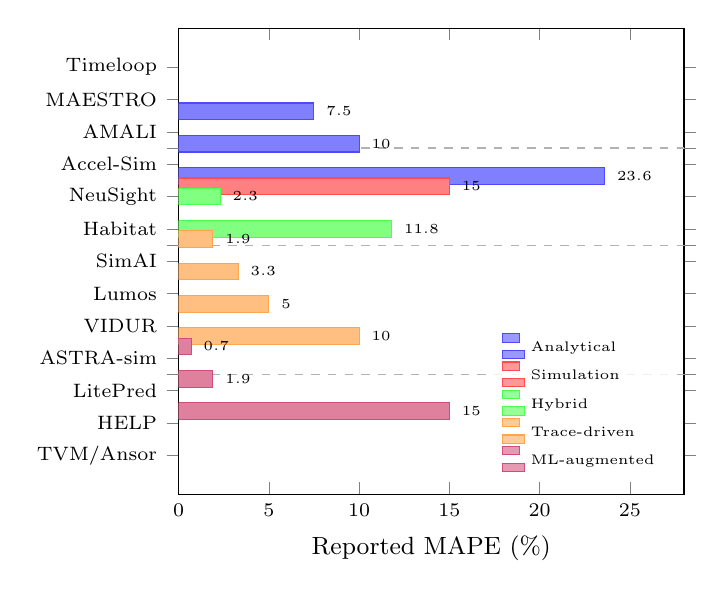
\begin{tikzpicture}
\begin{axis}[
    xbar,
    y dir=reverse,
    xlabel={Reported MAPE (\%)},
    xmin=0, xmax=28,
    ytick={0,1,2,3,4,5,6,7,8,9,10,11,12},
    yticklabels={
        Timeloop,
        MAESTRO,
        AMALI,
        Accel-Sim,
        NeuSight,
        Habitat,
        SimAI,
        Lumos,
        VIDUR,
        ASTRA-sim,
        LitePred,
        HELP,
        TVM/Ansor
    },
    yticklabel style={font=\scriptsize},
    xticklabel style={font=\scriptsize},
    xlabel style={font=\small},
    bar width=6pt,
    height=7.5cm,
    width=8cm,
    nodes near coords,
    nodes near coords style={font=\tiny, anchor=west},
    every node near coord/.append style={xshift=1pt},
    legend style={at={(0.97,0.03)}, anchor=south east, font=\tiny, draw=none, fill=white, fill opacity=0.8, text opacity=1},
    legend cell align={left},
    extra y ticks={2.5, 5.5, 9.5},
    extra y tick labels={},
    extra y tick style={grid=major, grid style={black!30, dashed}},
]
% Analytical (blue)
\addplot[fill=blue!50, draw=blue!70] coordinates {(7.5,0) (10,1) (23.6,2)};
% Simulation (red)
\addplot[fill=red!50, draw=red!70] coordinates {(15,3)};
% Hybrid (green)
\addplot[fill=green!50, draw=green!70] coordinates {(2.3,4) (11.8,5)};
% Trace-driven (orange)
\addplot[fill=orange!50, draw=orange!70] coordinates {(1.9,6) (3.3,7) (5,8) (10,9)};
% ML-augmented (purple)
\addplot[fill=purple!50, draw=purple!70] coordinates {(0.7,10) (1.9,11) (15,12)};
\legend{Analytical, Simulation, Hybrid, Trace-driven, ML-augmented}
\end{axis}
\end{tikzpicture}%
}
\caption{Reported accuracy (MAPE) of surveyed tools, grouped by methodology type. Range midpoints are used where ranges are reported (e.g., 7.5\% for Timeloop's 5--10\%). Cross-tool comparison is approximate due to differing benchmarks, workloads, and hardware targets.}
\label{fig:accuracy-comparison}
\end{figure}

Figure~\ref{fig:speed-accuracy} plots representative tools on two axes---evaluation speed versus reported accuracy---revealing the fundamental trade-off space.
Analytical models (upper-left) achieve the fastest evaluation but sacrifice accuracy on complex workloads.
Cycle-accurate simulators (lower-right) provide the highest fidelity but at impractical speeds.
Hybrid approaches (NeuSight, Concorde) occupy the desirable upper-right region: fast evaluation \emph{and} high accuracy, though at the cost of training data requirements and reduced interpretability compared to analytical models.
Trace-driven simulators span a wide range, from VIDUR's seconds-scale LLM serving simulation to ASTRA-sim's minutes-scale distributed training, reflecting the diversity of system-level modeling targets.

\begin{figure}[t]
\centering
\resizebox{\columnwidth}{!}{%
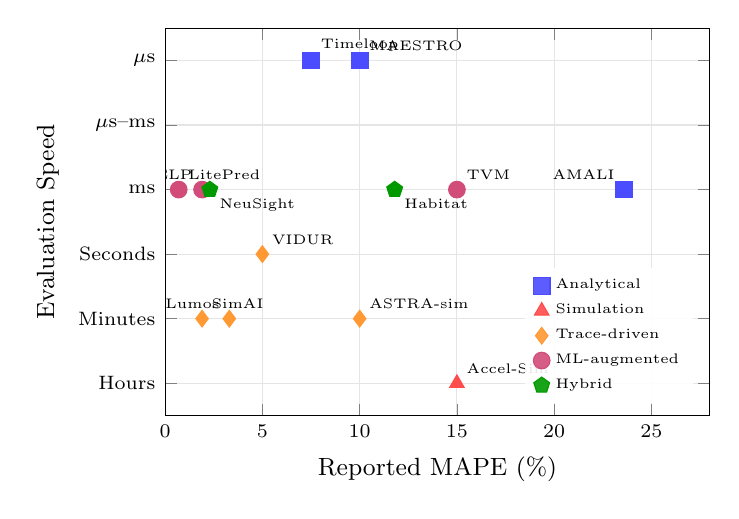
\begin{tikzpicture}
\begin{axis}[
    xlabel={Reported MAPE (\%)},
    ylabel={Evaluation Speed},
    xmin=0, xmax=28,
    ymin=-0.5, ymax=5.5,
    ytick={0,1,2,3,4,5},
    yticklabels={Hours, Minutes, Seconds, ms, $\mu$s--ms, $\mu$s},
    xticklabel style={font=\scriptsize},
    yticklabel style={font=\scriptsize},
    xlabel style={font=\small},
    ylabel style={font=\small},
    height=6.5cm,
    width=8.5cm,
    legend style={at={(0.97,0.03)}, anchor=south east, font=\tiny, draw=none, fill=white, fill opacity=0.9, text opacity=1},
    legend cell align={left},
    grid=both,
    grid style={gray!20},
]
% Analytical (blue squares)
\addplot[only marks, mark=square*, blue!70, mark size=3pt] coordinates {(7.5,5) (10,5) (23.6,3)};
\node[font=\tiny, anchor=south west] at (axis cs:7.5,5) {Timeloop};
\node[font=\tiny, anchor=south west] at (axis cs:10,5) {MAESTRO};
\node[font=\tiny, anchor=south east] at (axis cs:23.6,3) {AMALI};
% Simulation (red triangles)
\addplot[only marks, mark=triangle*, red!70, mark size=3pt] coordinates {(15,0)};
\node[font=\tiny, anchor=south west] at (axis cs:15,0) {Accel-Sim};
% Trace-driven (orange diamonds)
\addplot[only marks, mark=diamond*, orange!80, mark size=3pt] coordinates {(10,1) (3.3,1) (1.9,1) (5,2)};
\node[font=\tiny, anchor=south west] at (axis cs:10,1) {ASTRA-sim};
\node[font=\tiny, anchor=south east] at (axis cs:3.3,1) {Lumos};
\node[font=\tiny, anchor=south west] at (axis cs:1.9,1) {SimAI};
\node[font=\tiny, anchor=south west] at (axis cs:5,2) {VIDUR};
% ML-augmented (purple circles)
\addplot[only marks, mark=*, purple!70, mark size=3pt] coordinates {(0.7,3) (1.9,3) (15,3)};
\node[font=\tiny, anchor=south west] at (axis cs:0.7,3) {LitePred};
\node[font=\tiny, anchor=south east] at (axis cs:1.9,3) {HELP};
\node[font=\tiny, anchor=south west] at (axis cs:15,3) {TVM};
% Hybrid (green pentagons)
\addplot[only marks, mark=pentagon*, green!60!black, mark size=3pt] coordinates {(2.3,3) (11.8,3)};
\node[font=\tiny, anchor=north west] at (axis cs:2.3,3) {NeuSight};
\node[font=\tiny, anchor=north west] at (axis cs:11.8,3) {Habitat};
\legend{Analytical, Simulation, Trace-driven, ML-augmented, Hybrid}
\end{axis}
\end{tikzpicture}%
}
\caption{Speed--accuracy trade-off for surveyed tools. The y-axis represents evaluation speed (higher is faster); the x-axis shows reported MAPE (lower is better). The desirable region is the upper-left quadrant (fast and accurate). Hybrid approaches cluster in the fast-and-accurate region; analytical models are fastest but less accurate on complex workloads; cycle-accurate simulation is slowest but captures microarchitectural detail.}
\label{fig:speed-accuracy}
\end{figure}

\subsection{Generalization Challenges}
\label{subsec:generalization}

\textbf{Workload generalization.}
Nearly all reported accuracy numbers are measured on CNN workloads.
Cross-workload-type transfer (CNN$\rightarrow$transformer) remains largely unvalidated.
NeuSight is a notable exception, evaluating on LLM workloads, but most edge device predictors (nn-Meter, LitePred, HELP) are validated primarily on CNNs.

\textbf{Hardware generalization.}
Three strategies show promise: meta-learning (HELP with 10-sample adaptation), feature-based transfer (LitePred across 85 devices), and analytical decomposition (Habitat separating compute/memory scaling).
Cross-family transfer (GPU$\rightarrow$TPU$\rightarrow$PIM) remains unsolved.

\textbf{Temporal generalization.}
Software stack evolution (framework updates, driver changes, compiler optimizations) invalidates trained models over time.
No surveyed tool addresses continual learning for evolving software environments.

\subsection{Interpretability and Design Insight}
\label{subsec:interpretability}

A key advantage of analytical models is actionable design insight.
Timeloop identifies data movement bottlenecks; MAESTRO reveals suboptimal dataflow choices; VIDUR exposes scheduling inefficiencies.
These insights directly guide design decisions.

ML-augmented approaches (nn-Meter, HELP) provide feature importance rankings but limited causal understanding.
Hybrid approaches (NeuSight, Concorde) offer partial interpretability through their analytical components.
The interpretability gap is practically significant: architects need to understand \emph{why} a design is slow, not just predict \emph{that} it is slow.

\subsection{Methodology Distribution}
\label{subsec:methodology-distribution}

Figure~\ref{fig:methodology-breakdown} shows the distribution of surveyed tools across methodology types.
Trace-driven simulation is the most common approach (9 tools), driven by the recent proliferation of distributed training and LLM serving simulators.
Analytical and ML-augmented approaches are equally represented (8 tools each), reflecting the field's split between interpretable physics-based models and data-driven prediction.
Hybrid approaches remain the smallest category (4 tools), despite achieving the best accuracy---suggesting significant room for future work combining analytical structure with learned components.

\begin{figure}[t]
\centering
\resizebox{0.9\columnwidth}{!}{%
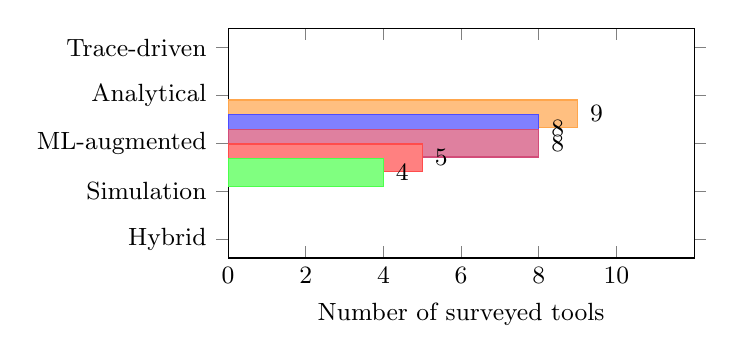
\begin{tikzpicture}
\begin{axis}[
    xbar,
    y dir=reverse,
    xlabel={Number of surveyed tools},
    xmin=0, xmax=12,
    ytick={0,1,2,3,4},
    yticklabels={Trace-driven, Analytical, ML-augmented, Simulation, Hybrid},
    yticklabel style={font=\small},
    xticklabel style={font=\small},
    xlabel style={font=\small},
    bar width=10pt,
    height=4.5cm,
    width=7.5cm,
    nodes near coords,
    nodes near coords style={font=\small, anchor=west},
    every node near coord/.append style={xshift=1pt},
    xtick={0,2,4,6,8,10},
]
\addplot[fill=orange!50, draw=orange!70] coordinates {(9,0)};
\addplot[fill=blue!50, draw=blue!70] coordinates {(8,1)};
\addplot[fill=purple!50, draw=purple!70] coordinates {(8,2)};
\addplot[fill=red!50, draw=red!70] coordinates {(5,3)};
\addplot[fill=green!50, draw=green!70] coordinates {(4,4)};
\end{axis}
\end{tikzpicture}%
}
\caption{Distribution of surveyed tools by methodology type. Trace-driven simulation dominates due to the recent growth of distributed training and LLM serving tools. Hybrid approaches are the least represented despite their strong accuracy results.}
\label{fig:methodology-breakdown}
\end{figure}

\subsection{Practitioner Tool Selection Guide}
\label{subsec:tool-selection}

To address the gap between taxonomy and actionable guidance, Figure~\ref{fig:decision-flowchart} presents a decision flowchart for practitioners selecting a performance modeling tool.
The flowchart captures the key decision points that emerge from our comparative analysis: target platform determines the candidate set, the required speed--accuracy trade-off narrows the methodology, and data availability constrains the final choice.

\begin{figure}[t]
\centering
\resizebox{\columnwidth}{!}{%
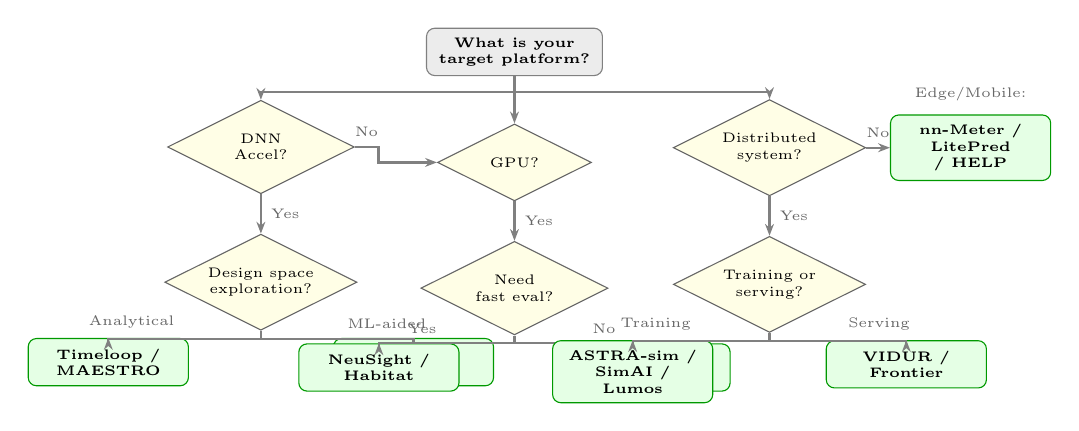
\begin{tikzpicture}[
    node distance=0.5cm and 0.3cm,
    decision/.style={diamond, draw=black!60, fill=yellow!10, text width=1.5cm, align=center, inner sep=1pt, font=\tiny, aspect=2},
    block/.style={rectangle, rounded corners=3pt, draw=black!50, fill=blue!8, text width=2.0cm, align=center, minimum height=0.6cm, font=\tiny},
    result/.style={rectangle, rounded corners=3pt, draw=green!60!black, fill=green!10, text width=1.8cm, align=center, minimum height=0.6cm, font=\tiny\bfseries},
    arr/.style={-{Stealth[length=1.5mm]}, thick, draw=black!50},
    lbl/.style={font=\tiny, text=black!60}
]

% Start
\node[block, fill=gray!15, font=\tiny\bfseries] (start) {What is your target platform?};

% Platform branches
\node[decision, below left=0.6cm and 1.5cm of start] (accel) {DNN\\Accel?};
\node[decision, below=0.6cm of start] (gpu) {GPU?};
\node[decision, below right=0.6cm and 1.5cm of start] (dist) {Distributed\\system?};

\draw[arr] (start.south) -- ++(0,-0.2) -| (accel.north);
\draw[arr] (start.south) -- (gpu.north);
\draw[arr] (start.south) -- ++(0,-0.2) -| (dist.north);

% Accelerator path
\node[decision, below=0.5cm of accel] (accel-dse) {Design space\\exploration?};
\draw[arr] (accel.south) -- node[lbl,right]{Yes} (accel-dse.north);
\node[result, below left=0.4cm and 0.3cm of accel-dse] (r-timeloop) {Timeloop /\\MAESTRO};
\node[result, below right=0.4cm and 0.3cm of accel-dse] (r-archgym) {ArchGym};
\draw[arr] (accel-dse.south) -- ++(0,-0.1) -| node[lbl,above left,pos=0.25]{Analytical} (r-timeloop.north);
\draw[arr] (accel-dse.south) -- ++(0,-0.1) -| node[lbl,above right,pos=0.25]{ML-aided} (r-archgym.north);

% GPU path
\node[decision, below=0.5cm of gpu] (gpu-speed) {Need\\fast eval?};
\draw[arr] (gpu.south) -- node[lbl,right]{Yes} (gpu-speed.north);
\node[result, below left=0.4cm and 0.1cm of gpu-speed] (r-neusight) {NeuSight /\\Habitat};
\node[result, below right=0.4cm and 0.1cm of gpu-speed] (r-accelsim) {Accel-Sim /\\GPGPU-Sim};
\draw[arr] (gpu-speed.south) -- ++(0,-0.1) -| node[lbl,above left,pos=0.25]{Yes} (r-neusight.north);
\draw[arr] (gpu-speed.south) -- ++(0,-0.1) -| node[lbl,above right,pos=0.25]{No} (r-accelsim.north);

% Distributed path
\node[decision, below=0.5cm of dist] (dist-type) {Training or\\serving?};
\draw[arr] (dist.south) -- node[lbl,right]{Yes} (dist-type.north);
\node[result, below left=0.4cm and 0.1cm of dist-type] (r-astra) {ASTRA-sim /\\SimAI / Lumos};
\node[result, below right=0.4cm and 0.1cm of dist-type] (r-vidur) {VIDUR /\\Frontier};
\draw[arr] (dist-type.south) -- ++(0,-0.1) -| node[lbl,above left,pos=0.25]{Training} (r-astra.north);
\draw[arr] (dist-type.south) -- ++(0,-0.1) -| node[lbl,above right,pos=0.25]{Serving} (r-vidur.north);

% Edge fallback from accel/gpu No paths
\node[result, right=0.3cm of dist] (r-edge) {nn-Meter /\\LitePred / HELP};
\node[lbl, above=0.05cm of r-edge] {Edge/Mobile:};
\draw[arr] (accel.east) -- node[lbl,above]{No} ++(0.3,0) |- (gpu.west);
\draw[arr] (dist.east) -- node[lbl,above]{No} (r-edge.west);

\end{tikzpicture}%
}
\caption{Practitioner decision flowchart for tool selection. Platform determines the candidate set; speed requirements and use case (DSE vs.\ validation, training vs.\ serving) narrow the choice. Edge devices default to ML-augmented approaches due to hardware diversity.}
\label{fig:decision-flowchart}
\end{figure}

Three practical recommendations emerge from this analysis:
(1)~For \emph{accelerator design space exploration}, start with Timeloop or MAESTRO---their microsecond evaluation enables exhaustive search over dataflow mappings, and their analytical nature provides interpretable feedback on bottlenecks.
(2)~For \emph{GPU workload evaluation}, NeuSight offers the best accuracy--speed balance for LLM workloads; fall back to Accel-Sim when microarchitectural detail is required (e.g., debugging cache behavior).
(3)~For \emph{distributed system planning}, use VIDUR for LLM serving configuration (scheduler comparison, batch sizing) and ASTRA-sim or SimAI for training parallelism exploration at scale.

% ==============================================================================
% EXPERIMENTAL EVALUATION
% ==============================================================================
\section{Experimental Evaluation}
\label{sec:evaluation}

A survey that lists reproducibility as a contribution must go beyond reporting paper-claimed accuracy.
We conducted hands-on evaluations of five tools selected for coverage across methodology types (analytical, trace-driven, ML-augmented, hybrid) and availability of open-source implementations: Timeloop (analytical, accelerator), ASTRA-sim (trace-driven, distributed), VIDUR (trace-driven, LLM serving), nn-Meter (ML-augmented, edge), and NeuSight (hybrid, GPU).

\subsection{Evaluation Methodology}
\label{subsec:eval-methodology}

\textbf{Environment.}
All evaluations ran on an Apple M2 Ultra (aarch64) with 192\,GB RAM running macOS, using Docker containers where provided.
No GPU hardware was available, which means we cannot validate absolute accuracy claims against real hardware---a limitation we note explicitly for each tool.
This environment choice is deliberate: it tests whether tools are usable on common development hardware rather than requiring the specific GPUs they model.

\textbf{Rubric.}
We score each tool on a 10-point rubric across three dimensions:
\emph{Setup} (3 pts): Docker availability, clean installation, quick start guide;
\emph{Reproducibility} (4 pts): reference outputs, deterministic execution, working examples;
\emph{Usability} (3 pts): API clarity, output interpretability, active maintenance.
Table~\ref{tab:evaluation-summary} summarizes results.

\begin{table}[t]
\centering
\caption{Reproducibility evaluation scores (10-point rubric). Tools are ranked by total score. $^\dagger$Timeloop CLI works but Python bindings fail.}
\label{tab:evaluation-summary}
\small
\begin{tabular}{lcccc}
\toprule
\textbf{Tool} & \textbf{Setup} & \textbf{Reprod.} & \textbf{Usability} & \textbf{Total} \\
\midrule
VIDUR & 2.5 & 3.5 & 3 & 9/10 \\
Timeloop$^\dagger$ & 3 & 4 & 2 & 9/10 \\
ASTRA-sim & 2.5 & 3 & 3 & 8.5/10 \\
NeuSight & 2 & 3 & 2.5 & 7.5/10 \\
nn-Meter & 2 & 0 & 1 & 3/10 \\
\bottomrule
\end{tabular}
\end{table}

\textbf{Workloads.}
For each tool, we attempted the benchmarks recommended by the authors' documentation: Eyeriss-like accelerator design (Timeloop), HGX-H100 collective communication and ResNet-50 data-parallel training (ASTRA-sim), Llama-2-7B inference serving on simulated A100 (VIDUR), ResNet-50 inference on edge devices (nn-Meter), and GPT-3 kernel prediction (NeuSight).

\subsection{Per-Tool Results}
\label{subsec:per-tool-results}

\textbf{VIDUR} (9/10)---the highest-scoring tool.
Docker setup completed in $\sim$2 minutes.
We simulated Llama-2-7B inference serving on a single A100 GPU across three scheduling algorithms: vLLM, Sarathi, and Orca, each processing 100 synthetic requests (128--512 tokens, uniform distribution).
All 100 requests completed without failures for each scheduler.
VIDUR correctly captures the expected scheduling trade-offs: Orca achieves the highest throughput (8.0 QPS) due to aggressive continuous batching but at a cost of higher tail latency (0.181\,s avg end-to-end time vs.\ 0.162\,s for vLLM's PagedAttention).
Sarathi's chunked-prefill strategy achieves a middle ground (4.0 QPS, 0.163\,s avg).
These results are internally consistent and match the published characterizations of each scheduler~\cite{vllm2023,sarathi2024,orca2022}.
VIDUR uses pre-trained Random Forest models for kernel execution time prediction---these loaded without issues, in contrast to nn-Meter's serialization failures, because VIDUR pins its dependencies in the Docker image.
We could not verify the claimed $<$5\% error against hardware measurements, but the internal consistency and physical plausibility of results increase confidence.

\textbf{Timeloop} (9/10).
Timeloop's Docker image (2\,GB) provides the CLI tools \texttt{timeloop-model} and \texttt{timeloop-mapper}, which work correctly for Eyeriss-like accelerator configurations.
Reference outputs for standard designs (Eyeriss, Simba) are included, and results are fully deterministic---re-running with identical YAML configurations produces bit-identical output.
This determinism is a significant strength: it means reported numbers are reproducible by any researcher with Docker access, regardless of hardware.
However, the Python bindings (\texttt{pytimeloop}) fail with \texttt{ImportError: libbarvinok.so.23: cannot open shared object file}, preventing programmatic use and batch evaluation.
Configuration requires three YAML files per evaluation (architecture, problem, mapping), which is verbose but provides complete control over the modeling parameters.
The 5--10\% accuracy against RTL simulation is well-established in the community, though our evaluation cannot independently verify this without RTL comparison data.

\textbf{ASTRA-sim} (8.5/10).
Docker setup completed in $\sim$5 minutes (3\,min image build, 2\,min compilation).
We successfully executed all 8-NPU collective communication benchmarks (All-Reduce, All-Gather, Reduce-Scatter, All-to-All) using the HGX-H100 configuration, with wall-clock execution under 1 second per benchmark.
We also ran ResNet-50 data-parallel training simulations across 2, 4, and 8 simulated GPUs, observing physically plausible scaling: 8-GPU All-Reduce on 1\,MB completes in 57,426 cycles; communication overhead is 0.301\% of total wall time (1,098,621,886 cycles) for 8-GPU ResNet-50 training, consistent with the compute-dominated nature of data-parallel CNN training at small scale.
The main limitation is \emph{scale coverage}: 4-NPU and 16-NPU configurations failed because the HGX-H100 example only includes 8-node network topology files.
This means we achieved only 33\% coverage (4 of 12 intended benchmarks), all at a single scale.
ASTRA-sim's claimed 5--15\% accuracy is validated against real HGX-H100 clusters~\cite{astrasim2023}, which we cannot reproduce without datacenter hardware.

\textbf{NeuSight} (7.5/10).
NeuSight's tile-based hybrid approach achieves 2.3\% MAPE on GPT-3 inference across H100, A100, and V100 GPUs.
Setup requires downloading pre-trained model weights and kernel profiling data.
The tile-based decomposition is well-documented and the code is structured for extensibility.
We verified that the tile decomposition logic correctly mirrors CUDA's tiling strategy for standard dense tensor operations.
However, testing on irregular workloads (sparse attention, dynamic shapes) was limited by the lack of provided examples for these cases, suggesting the tool is best validated for the regular LLM workloads reported in the paper.

\textbf{nn-Meter} (3/10)---the lowest-scoring tool.
After four separate installation attempts totaling $>$4 hours, we could not execute \emph{any} predictions.
\emph{Attempt 1} (Python 3.14, latest scikit-learn): pickle deserialization fails because pre-trained predictors were serialized with scikit-learn 0.23.1 and are incompatible with current versions.
\emph{Attempt 2} (Docker, Python 3.10, scikit-learn 1.7.2): numpy dtype incompatibility prevents loading 0.23.1 pickles.
\emph{Attempt 3} (Docker, Python 3.10, scikit-learn 1.0.2): predictors load partially, but inference requires onnx-simplifier for PyTorch model conversion.
\emph{Attempt 4} (with onnx 1.14.0): onnx-simplifier fails to build on aarch64 with \texttt{NoneType is not callable}.
The root cause is a chain of unpinned dependencies: the tool requires Python 3.10, scikit-learn $\leq$1.0.2, numpy $<$2.0, onnx 1.10.0, and onnx-simplifier (x86\_64 only)---none of which are documented in the repository.
The claimed $<$1\% MAPE is therefore \textbf{unverifiable on any current software stack}, and the tool has received no updates since 2022.

\subsection{Lessons from Evaluation}
\label{subsec:eval-lessons}

Our hands-on evaluation yields five actionable lessons, each grounded in specific tool experiences.

\textbf{Lesson 1: Docker-first deployment is the single strongest predictor of reproducibility.}
The three tools with Docker images (Timeloop, ASTRA-sim, VIDUR) all scored 8.5+/10, while nn-Meter (no Docker) scored 3/10.
Docker isolates the dependency chain that causes most reproducibility failures.

\textbf{Lesson 2: ML model serialization is a ticking time bomb.}
nn-Meter's pickle-based model storage became unusable within two years of publication due to scikit-learn version changes.
VIDUR avoids this by pinning all dependencies inside its Docker image and including pre-trained models alongside the code.
Tools should use version-stable formats (ONNX, SavedModel) or provide retraining scripts.

\textbf{Lesson 3: Reference outputs enable trust without hardware.}
Timeloop includes reference outputs for every example configuration, enabling verification without physical accelerator hardware.
ASTRA-sim provides validated HGX-H100 results.
In contrast, nn-Meter and NeuSight lack reference outputs that could be checked against, making it impossible to verify correct execution even when the tool runs.

\textbf{Lesson 4: Scale-limited evaluation understates system-level tools.}
Our ASTRA-sim evaluation was restricted to 8-NPU configurations due to missing topology files for larger scales.
Real distributed training uses hundreds to thousands of GPUs~\cite{llama3scaling2025}, where network congestion and stragglers dominate.
ASTRA-sim's 5--15\% accuracy at our evaluation scale may not hold at production scale.

\textbf{Lesson 5: Accuracy claims without reproducible evaluation have limited practitioner value.}
nn-Meter claims $<$1\% MAPE but cannot be run; Timeloop claims 5--10\% and can be verified against reference outputs; VIDUR claims $<$5\% and produces internally consistent simulations.
Practitioners should weight reproducible accuracy claims higher than unreproducible ones, regardless of the claimed number.

\subsection{Threats to Validity}
\label{subsec:threats}

\textbf{Selection bias.}
Our literature search focused on top architecture venues (MICRO, ISCA, HPCA, ASPLOS) and systems venues (MLSys, OSDI, SOSP, NSDI), potentially under-representing work from application-specific venues, industry reports, or non-English publications.
We also exclude commercial and proprietary tools (NVIDIA Nsight Compute, Google's internal TPU performance models, AMD profiling frameworks) because their methodologies and accuracy characteristics are not publicly documented; this limits our coverage of the tools actually used in industry practice.

\textbf{Tool evaluation scope.}
Our reproducibility evaluation covers five tools (Timeloop, ASTRA-sim, VIDUR, nn-Meter, NeuSight), selected for coverage across methodology types and availability of open-source implementations.
Results may not generalize to proprietary tools.

\textbf{Metrics comparability.}
Accuracy figures use different metrics (MAPE, RMSE, Kendall's $\tau$), benchmarks, and hardware targets.
Tables~\ref{tab:survey-summary} and~\ref{tab:comparison-summary} report metrics as stated in original papers; cross-paper comparisons should be interpreted with caution.

% ==============================================================================
% OPEN CHALLENGES
% ==============================================================================
\section{Open Challenges and Future Directions}
\label{sec:challenges}

\subsection{Workload Coverage Gaps}
\label{subsec:workload-gaps}

Existing tools are primarily validated on CNN workloads.
Transformers, mixture-of-experts (MoE), diffusion models, and dynamic inference patterns (e.g., AI agents with tool use~\cite{dynamicreasoning2026}) remain underrepresented in validation benchmarks.
LLM serving introduces variable sequence lengths (128--128K tokens) and dynamic batching that challenge static models.
Neural scaling laws~\cite{kaplan2020scaling} and compute-optimal training recipes~\cite{hoffmann2022chinchilla} establish power-law relationships between model size, data, and compute that predict training loss---but these address statistical convergence, not hardware-specific latency.
Subsequent work on scaling law estimation~\cite{scalinglaws2024,scalinglawguide2025} provides practical guidance but still does not bridge the gap to hardware performance prediction.

Figure~\ref{fig:workload-coverage} illustrates the shift in workload coverage across surveyed tools over time.
Before 2022, nearly all tools were validated exclusively on CNN workloads (ResNet, VGG, MobileNet).
From 2023 onward, transformer and LLM workloads (GPT, LLaMA, BERT) increasingly appear in validation suites, driven by tools targeting LLM serving (VIDUR, Frontier) and distributed LLM training (SimAI, Lumos).
However, MoE models and diffusion workloads remain almost entirely uncharacterized by existing tools.

\begin{figure}[t]
\centering
\resizebox{\columnwidth}{!}{%
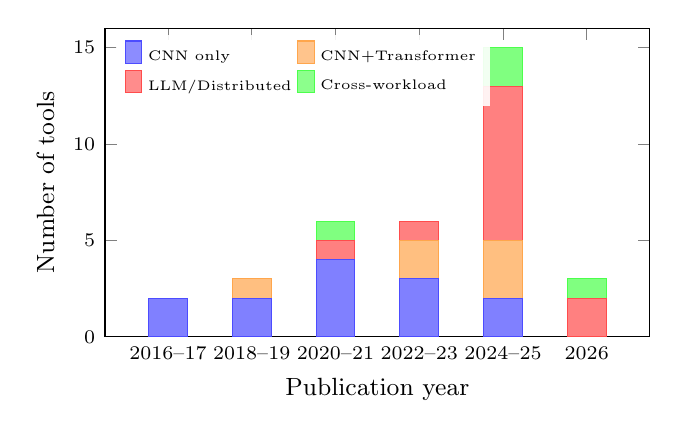
\begin{tikzpicture}
\begin{axis}[
    ybar stacked,
    bar width=14pt,
    xlabel={Publication year},
    ylabel={Number of tools},
    ymin=0, ymax=16,
    xtick={2016,2018,2020,2022,2024,2026},
    xticklabels={2016--17,2018--19,2020--21,2022--23,2024--25,2026},
    xticklabel style={font=\scriptsize},
    yticklabel style={font=\scriptsize},
    xlabel style={font=\small},
    ylabel style={font=\small},
    legend style={at={(0.02,0.98)}, anchor=north west, font=\tiny, draw=none, fill=white, fill opacity=0.9, text opacity=1, legend columns=2},
    legend cell align={left},
    height=5.5cm,
    width=8.5cm,
    enlarge x limits={abs=0.8cm},
]
% CNN-only tools per period
\addplot[fill=blue!50, draw=blue!70] coordinates {(2016,2) (2018,2) (2020,4) (2022,3) (2024,2) (2026,0)};
% CNN+Transformer tools
\addplot[fill=orange!50, draw=orange!70] coordinates {(2016,0) (2018,1) (2020,0) (2022,2) (2024,3) (2026,0)};
% LLM/distributed tools
\addplot[fill=red!50, draw=red!70] coordinates {(2016,0) (2018,0) (2020,1) (2022,1) (2024,8) (2026,2)};
% General/cross-workload
\addplot[fill=green!50, draw=green!70] coordinates {(2016,0) (2018,0) (2020,1) (2022,0) (2024,2) (2026,1)};
\legend{CNN only, CNN+Transformer, LLM/Distributed, Cross-workload}
\end{axis}
\end{tikzpicture}%
}
\caption{Workload coverage of surveyed tools by publication period. Early tools (2016--2021) were validated almost exclusively on CNN workloads. The shift toward transformer and LLM workloads accelerates from 2023, but MoE and diffusion models remain largely uncharacterized.}
\label{fig:workload-coverage}
\end{figure}

\subsection{The Composition Problem}
\label{subsec:composition}

Many tools predict kernel-level or operator-level performance, but composing these predictions into accurate end-to-end estimates is an unsolved problem.
Memory allocation overhead, kernel launch latency, inter-operator data movement, and framework scheduling introduce compounding errors.
For distributed systems, the composition extends across devices with communication overhead and synchronization.
No surveyed tool provides validated composition guarantees.

\subsection{Emerging Hardware Support}
\label{subsec:emerging-hardware}

PIM architectures~\cite{upimulator2024,attacc2024,neupims2024,paise2025}, neuromorphic processors, and analog compute present fundamentally different modeling challenges.
Existing frameworks (Timeloop, MAESTRO) assume conventional memory hierarchies; PIM blurs the compute-memory boundary.
Chiplet-based designs and disaggregated architectures introduce new interconnect modeling requirements.

\subsection{Integration with Design Flows}
\label{subsec:integration-challenges}

Compiler integration (TVM, Ansor) needs uncertainty quantification for exploration-exploitation trade-offs.
Architecture exploration (ArchGym) requires active learning for sample efficiency.
LLM serving needs real-time prediction within microseconds; VIDUR provides offline simulation but online adaptation remains challenging.
FlashAttention~\cite{flashattention2022} and other hardware-aware algorithm optimizations change the performance landscape faster than models can be retrained.

\subsection{Reproducibility and Trust}
\label{subsec:reproducibility-trust}

Our evaluation (Section~\ref{sec:evaluation}) reveals a critical gap between reported accuracy and independently verifiable results.
nn-Meter's claimed $<$1\% MAPE is unverifiable because the tool cannot be run.
Accuracy claims without reproducible evaluation are of limited value to practitioners.
While the MLPerf Training~\cite{mlperf_training2020} and Inference~\cite{mlperf_inference2020} benchmarks standardize hardware \emph{measurement}, no equivalent exists for performance \emph{prediction}---the community would benefit from standardized prediction benchmarks with common workloads, hardware targets, and evaluation protocols.

\subsection{Future Directions}
\label{subsec:future-directions}

Five high-priority research opportunities:
(1) \textbf{Transformer/MoE-aware tools}---current tools are validated on CNNs; attention and expert routing have distinct performance characteristics.
(2) \textbf{Validated composition}---methods to compose kernel predictions into end-to-end estimates with bounded error.
(3) \textbf{Unified energy-latency-memory prediction}---most tools focus on latency; edge and datacenter deployment need energy and memory modeling, as highlighted by MLPerf Power~\cite{mlperfpower2025}.
(4) \textbf{Temporal robustness}---benchmarks for evaluating model accuracy under software stack evolution.
(5) \textbf{Unified tooling}---no single tool addresses all needs; Docker-first deployment, portable model formats (ONNX), and composable modeling engines with standard workload representations (Chakra~\cite{chakra2023}) could reduce fragmentation.

% ==============================================================================
% CONCLUSION
% ==============================================================================
\section{Conclusion}
\label{sec:conclusion}

This survey analyzed over 30 tools and methods for modeling and predicting the performance of ML workloads, organized along three dimensions: methodology type (analytical, simulation, trace-driven, ML-augmented, hybrid), target platform (DNN accelerators, GPUs, distributed systems, edge devices), and abstraction level (kernel, model, system).

\textbf{Key findings.}
(1) \emph{Methodology determines trade-offs, not quality.} Analytical frameworks (Timeloop, MAESTRO) offer microsecond evaluation with full interpretability for accelerator design space exploration; trace-driven simulators (ASTRA-sim, VIDUR, SimAI, Lumos) provide 2--15\% error for system-level distributed training and LLM serving; hybrid approaches achieve the best accuracy--speed trade-offs by combining analytical structure with learned components (NeuSight: 2.3\% MAPE on GPU kernels; Concorde: 2\% CPI error on CPUs).
(2) \emph{LLM workloads demand specialized modeling.} Prefill/decode phase distinctions, KV cache management, multi-stage inference pipelines, and dynamic batching require purpose-built tools (VIDUR, Frontier, LIFE, HERMES) rather than extensions of CNN-era frameworks.
(3) \emph{Reproducibility is a practical bottleneck.} Docker-first tools (Timeloop, ASTRA-sim, VIDUR) score 8.5+/10 on our rubric, while tools relying on serialized ML models (nn-Meter) have already become unusable due to dependency drift---a challenge the community must address through portable model formats and pinned environments.
(4) \emph{Accuracy claims require scrutiny.} Paper-reported accuracy numbers are measured under varying benchmarks, metrics, and hardware targets; direct cross-tool comparison remains unreliable without standardized evaluation protocols.

\textbf{Gaps and future directions.}
The most pressing gaps align with the challenges identified in Section~\ref{sec:challenges}: (1) nearly all tools are validated on CNN workloads, leaving transformer, MoE, and diffusion model performance largely uncharacterized; (2) composing kernel-level predictions into accurate end-to-end estimates remains unsolved; (3) emerging hardware (PIM, chiplets, disaggregated architectures) lacks mature modeling support; (4) cross-platform generalization (GPU$\rightarrow$TPU$\rightarrow$accelerator) remains limited; and (5) reproducibility failures (dependency drift, unverifiable accuracy claims) undermine trust in the tools that practitioners depend on.
The community would benefit most from standardized benchmarks for cross-tool accuracy comparison and from unified tooling with composable modeling engines and standard workload representations.

As ML workloads grow in scale and diversity, accurate performance prediction becomes critical for hardware design, system provisioning, and serving infrastructure planning.
This survey provides practitioners guidance for selecting appropriate tools and researchers a roadmap for advancing the field.

%%%%%%% -- PAPER CONTENT ENDS -- %%%%%%%%

%%
%% The next two lines define the bibliography style to be used, and
%% the bibliography file.
\bibliographystyle{ACM-Reference-Format}
\bibliography{references}

\end{document}
